% Pulse selection and cubic-spline template fit for the PRad-II HyCal PbWO4 waveforms.
% Describes waveform_analysis/template_extract.py (branch waveform_jz).
% Section -> function map (for the reader who wants the code):
%   2  Selector.flush, _scan_events, pulse_features, cfd_onset
%   3  energy_pools
%   4  PulseSet, pool_points
%   5  knot_plan, tail_extension, _penalty
%   6  fit_spline, finalize_spline, bin_stats, align_pulses, _chi2_at, build_shape,
%      fit_module, _chi2_full, _osc_count
%   7  template_rows, band_stats, shape_sigma, _gsigma
%   8  process_module, run_average
%   9  the npz / ROOT writer and example_pulses
\documentclass[11pt]{article}
\usepackage[a4paper,margin=25mm]{geometry}
\usepackage{amsmath}
\usepackage{amssymb}
\usepackage{booktabs}
\usepackage{graphicx}
\graphicspath{{figs/}}
\usepackage[colorlinks=true,linkcolor=blue,urlcolor=blue]{hyperref}

\newcommand{\ns}{\,\mathrm{ns}}
\newcommand{\adc}{\,\mathrm{ADC}}
\newcommand{\code}[1]{\texttt{#1}}
\DeclareMathOperator*{\argmin}{arg\,min}
\DeclareMathOperator*{\argmax}{arg\,max}
\DeclareMathOperator{\median}{median}
\DeclareMathOperator{\MAD}{MAD}
\DeclareMathOperator{\sgn}{sgn}

\title{Pulse selection and cubic-spline pulse templates\\ for the HyCal PbWO$_4$ waveforms}
\author{PRad-II waveform analysis}
\date{\today}

\begin{document}
\maketitle

\section{Notation}

Each PbWO$_4$ channel is read out as 100 flash-ADC samples at a 4\,ns period. The symbols below are used throughout; every other symbol is defined where it first appears.

\begin{center}
\begin{tabular}{lp{0.72\textwidth}}
\toprule
Symbol & Meaning \\
\midrule
$s_{ij}$ & raw ADC sample $j = 0,\dots,99$ of pulse $i$ \\
$t_j = 4j\ns$ & sample time \\
$p_i$, $r_i$ & WaveAnalyzer pedestal and pedestal rms of pulse $i$ (ADC) \\
$n_{\mathrm{ped}}$ & number of samples in the WaveAnalyzer pedestal window \\
$w_{ij} = s_{ij} - p_i$ & baseline-subtracted sample \\
$k_i$ & peak sample, the first index at which $w_{ij}$ reaches its maximum \\
$A_i$ & pulse amplitude; at selection $A_i^{\mathrm{raw}} = w_{ik_i}$, in the fit the fitted amplitude \\
$\sigma_i = \max(r_i,\,0.3\adc)$ & per-sample noise of pulse $i$ (\code{SIG\_MIN}) \\
$E_b$ & beam energy (MeV); $c_m$ the calibration constant of module $m$ (MeV per ADC sample) \\
$t_{0,i}$ & pulse onset (ns); $t^{\mathrm{cfd}}_i$ its first estimate from a constant-fraction crossing \\
$\tau_{ij} = t_j - t_{0,i}$ & sample time relative to the onset \\
$f(\tau)$ & unit-peak template of a module; $f_{\mathrm{ref}}$ the template of the previous fit pass \\
$\lambda$ & smoothing parameter of the spline fit \\
\bottomrule
\end{tabular}
\end{center}

\section{Pulse selection}
\label{sec:selection}

Selection runs on the decoded events of one run and stores, for each surviving pulse, its 100 samples, pedestal, rms, amplitude, peak sample, onset estimate and rough energy. The event-level gates come first; the per-pulse cuts follow in the order of Table~\ref{tab:cuts}.

\subsection{Event-level gates}

An event enters the selection when all of the following hold.
\begin{enumerate}
\item \textbf{Trigger.} Run types with the \code{physics} trigger rule require $\code{trigger\_bits} = \code{0x100}$ exactly; run types with \code{physics-any} require $(\code{trigger\_bits}\ \&\ \code{0xf00}) \neq 0$.
\item \textbf{No LMS.} An event with bit \code{0x1000000} set in \code{trigger\_bits} is dropped (\code{EXCLUDE\_TRIGGER\_BITS}).
\item \textbf{Channel.} Only channels mapped to a HyCal PbWO$_4$ module that is not in the dead list, with exactly 100 samples, are kept.
\item \textbf{Busy event.} Over the channels of the event, count those with $\max_j s_{ij} - p_i \ge 50\adc$ (\code{MODULE\_COUNT\_HEIGHT\_MIN}). If more than 20 channels qualify (\code{MAX\_MODULES\_PER\_EVENT}) the whole event is dropped. This count uses the raw maximum, so clipped channels are included, and the gate precedes the clipping cut.
\end{enumerate}

\subsection{Per-pulse cuts}

The pedestal $p_i$ and rms $r_i$ are the WaveAnalyzer values of the pulse itself. The cuts of Table~\ref{tab:cuts} are boolean masks combined by logical AND, so the set of surviving pulses does not depend on their order; the order fixes only the cumulative cut-flow counters.

\begin{table}[htbp]
\centering
\caption{Per-pulse selection cuts in code order. $A_i = A^{\mathrm{raw}}_i$ throughout this table.}
\label{tab:cuts}
\small
\begin{tabular}{llll}
\toprule
\# & Cut & Condition & Constant \\
\midrule
1 & no clipping & $\max_j s_{ij} < 4095$ & \code{CLIP\_ADC} \\
2 & amplitude & $A_i = \max_j s_{ij} - p_i \ge 50\adc$ & \code{A\_STORE\_MIN} \\
3 & contained & $k_i \le 59$ & \code{PEAK\_MAX\_SAMPLE} \\
4 & pre-pulse window & $j^{\mathrm{thr}}_i \ge 20$ & \code{PRE\_SAMPLES}, \code{THR\_ADC} \\
5 & pedestal quality & $r_i \le 1.5\adc$ and $|b_i| \le 0.05\adc/\text{sample}$ & \code{PED\_RMS\_MAX}, \code{PED\_SLOPE\_MAX} \\
6 & tail level & $|\bar w^{\mathrm{tail}}_i| \le \max(2\adc,\,2r_i) + 0.04\,A_i$ & \code{TAIL\_*} \\
7 & no secondary bump & $\beta_i < 0.10\,A_i$ & \code{SEC\_FRAC} \\
8 & smoothness & rising edge monotone, tail steps $\le 2 r_i$ & \code{TAIL\_NSAMP}, \code{NOISE\_ALLOW} \\
9 & energy & $e^{\mathrm{rough}}_i < 1.2\,E_b$ & \code{EMAX\_FRAC} \\
\bottomrule
\end{tabular}
\end{table}

The quantities in the table are defined as follows. Cuts 4 to 8 act on $w_{ij}$, computed for the pulses that passed cuts 1 to 3.

\paragraph{Pre-pulse window (cut 4).} $j^{\mathrm{thr}}_i$ is the first sample at or before the peak that exceeds 2\,ADC above the pedestal:
\begin{equation}
j^{\mathrm{thr}}_i = \min\{\, j \le k_i : w_{ij} > 2\adc \,\}.
\end{equation}
Requiring $j^{\mathrm{thr}}_i \ge 20$ guarantees 20 pre-pulse samples.

\paragraph{Pedestal quality (cut 5).} The pre-pulse slope $b_i$ is the least-squares slope of the 20 samples before $j^{\mathrm{thr}}_i$,
\begin{equation}
b_i = \frac{\sum_{l=0}^{19} x_l\, w_{i,\,j^{\mathrm{thr}}_i - 20 + l}}{\sum_{l=0}^{19} x_l^2},
\qquad x_l = l - 9.5,
\end{equation}
in ADC per sample. The slope is evaluated only for pulses that passed cut 4.

\paragraph{Tail level (cut 6).} $\bar w^{\mathrm{tail}}_i$ is the mean of $w_{ij}$ over the samples $k_i + 40 \le j \le \min(k_i + 50,\, 99)$ (\code{TAIL\_OFF0}, \code{TAIL\_OFF1}). The tolerance $\max(2\adc, 2r_i) + 0.04\,A_i$ combines the noise floor with a 4\,\% allowance for the pulse's own tail (\code{TAIL\_ABS\_ADC}, \code{TAIL\_RMS\_MULT}, \code{TAIL\_FRAC\_A}).

\paragraph{Secondary bump (cut 7).} $\beta_i$ is the largest rise of any post-peak sample above the lowest sample seen since the peak,
\begin{equation}
\beta_i = \max_{j > k_i}\Big[\, w_{ij} - \min_{k_i \le l \le j} w_{il} \,\Big].
\end{equation}
A pile-up pulse in the tail raises $\beta_i$ by its own amplitude; the cut rejects anything above 10\,\% of $A_i$.

\paragraph{Smoothness (cut 8).} Let $j^{\mathrm{edge}}_i = 1 + \max\{ j < k_i : w_{ij} \le 2\adc \}$ be the sample after the last sub-threshold sample before the peak. The rising edge must not decrease,
\begin{equation}
w_{i,j+1} \ge w_{ij} \quad \text{for } j^{\mathrm{edge}}_i \le j < k_i,
\end{equation}
and over the eight samples after the peak no sample may rise above its predecessor by more than twice the noise,
\begin{equation}
w_{i,j+1} - w_{ij} \le 2\,r_i \quad \text{for } k_i \le j < k_i + 8 .
\end{equation}

\paragraph{Onset and rough energy.} For the pulses that passed cuts 1 to 8 the constant-fraction onset is the linearly interpolated time at which the rising edge first reaches half the amplitude (\code{CFD\_FRAC}),
\begin{equation}
t^{\mathrm{cfd}}_i = 4\ns\,\Big[(q-1) + \frac{0.5\,A_i - w_{i,q-1}}{w_{iq} - w_{i,q-1}}\Big],
\qquad q = \min\{\, j : w_{ij} \ge 0.5\,A_i \,\}.
\label{eq:cfd}
\end{equation}
The rough energy sums the baseline-subtracted samples from three samples before the onset sample to the end of the window (\code{E\_PRE}),
\begin{equation}
e^{\mathrm{rough}}_i = c_m \sum_{j \ge \lfloor t^{\mathrm{cfd}}_i / 4\ns \rfloor - 3}^{99} w_{ij}.
\label{eq:erough}
\end{equation}
Cut 9 keeps $e^{\mathrm{rough}}_i < 1.2\,E_b$.

\paragraph{Cut flow.} Per module, the selection records the number of pulses surviving each cut cumulatively in code order. No per-module cap is applied at selection. Pile-up is removed only by the shape cuts 6 to 8.

\section{Fit pool per module}
\label{sec:pools}

The template of module $m$ is fitted to a pool of its selected pulses. Pulses are sorted by $e^{\mathrm{rough}}$ in descending order, and one random generator per module, seeded with $(1, m)$ (\code{SEED}), draws every random subset. Let $n_{\mathrm{el}}$ be the number of pulses with $e^{\mathrm{rough}} \ge 0.5\,E_b$ (\code{POOL\_EFRAC}): the seed crystal of an elastic cluster holds about 70\,\% of the energy. The candidate pools are tried in the following order until the fit of Section~\ref{sec:fit} succeeds.

\begin{enumerate}
\item \textbf{Elastic}, if $n_{\mathrm{el}} \ge 20$ (\code{POOL\_MIN\_EP}). If $n_{\mathrm{el}} > 1000$ (\code{POOL\_MAX}) a random subset of 1000 pulses is drawn without replacement; the surplus is not used. The held-out set for the choice of $\lambda$ consists of the next $\lfloor 0.25\, n_{\mathrm{used}} + 0.5 \rfloor$ pulses below the threshold in $e^{\mathrm{rough}}$, where $n_{\mathrm{used}}$ is the pool size after the cap (\code{HOLDOUT\_FRAC} $=0.2$ of pool plus held-out).
\item \textbf{General}, if at least 20 pulses (\code{POOL\_MIN\_GEN}) have $200\adc \le A^{\mathrm{raw}} \le 1000\adc$ (\code{A\_LO}, \code{A\_HI}). The band is randomly permuted; the first $n_{\mathrm{used}} = \min(1000, \lfloor 0.8\, n_{\mathrm{band}} + 0.5 \rfloor)$ pulses form the pool and the next $\lfloor 0.25\, n_{\mathrm{used}} + 0.5 \rfloor$ are held out.
\item \textbf{Small elastic}, if $3 \le n_{\mathrm{el}} < 20$, with the same held-out rule.
\item \textbf{Single}: the pulse of largest amplitude; no held-out set.
\end{enumerate}
A module whose pools all fail, or that has no pulse at all, receives the run-type average of Section~\ref{sec:fallback}. Figure~\ref{fig:poolmap} shows the pool kind and size of every module for one run type.

\begin{figure}[htbp]
\centering
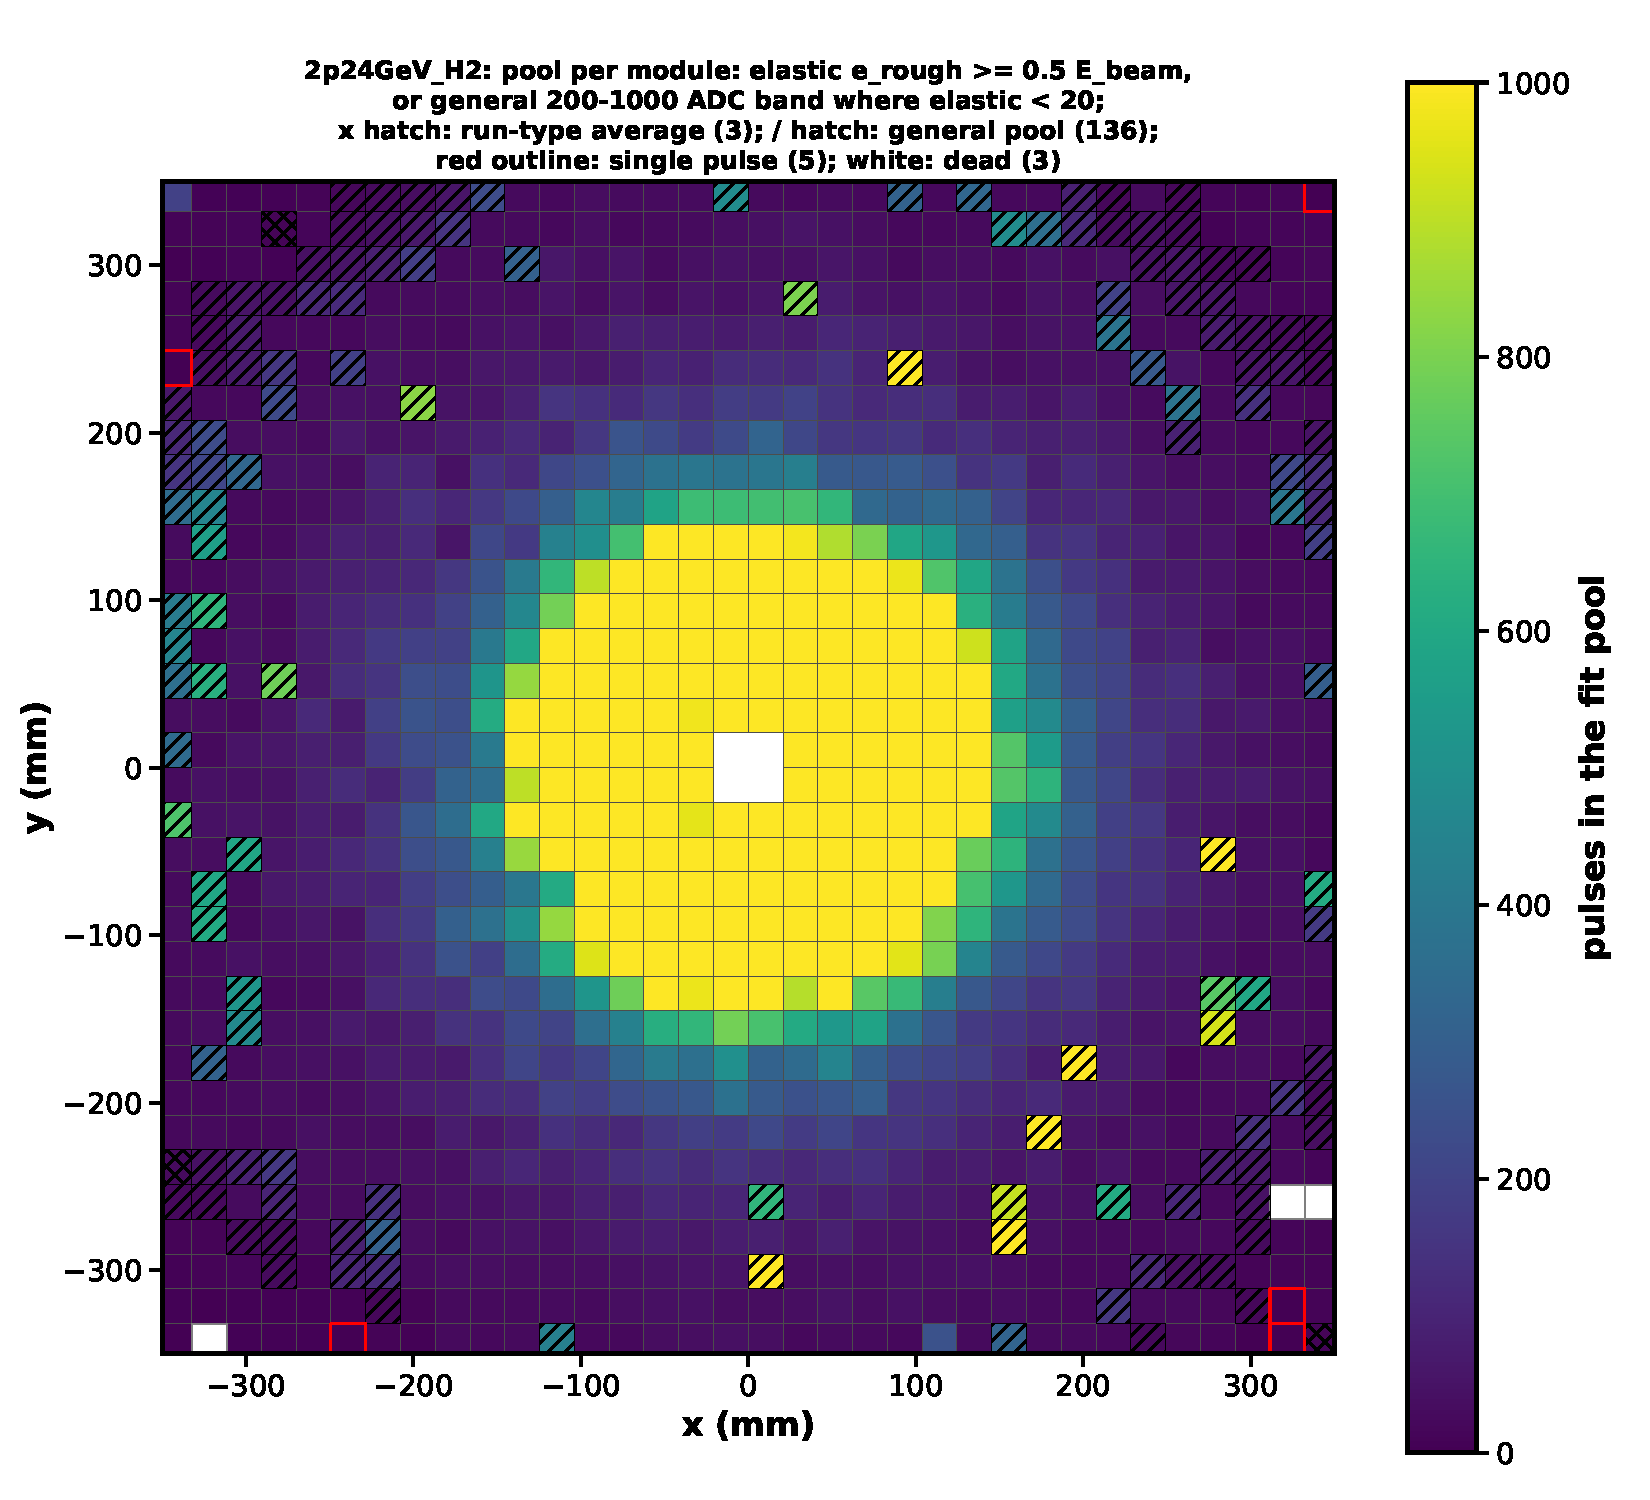
\includegraphics[width=0.85\textwidth]{summary_pool_map.pdf}
\caption{Fit-pool size per module for the \code{2p24GeV\_H2} build. Each rectangle sits at the module's HyCal position ($x$ and $y$ in mm); the colour gives the number of pulses in the fit pool, capped at 1000. Cross hatching marks modules with the run-type average, slash hatching general-pool modules, a red outline single-pulse modules, and white dead modules. The title states the pool rule and the module counts.}
\label{fig:poolmap}
\end{figure}

\section{Per-pulse preprocessing}
\label{sec:prep}

Each pooled pulse is baseline-subtracted with its WaveAnalyzer pedestal, $y_{ij} = s_{ij} - p_i$; no pedestal refit and no slope correction are applied. The time axis of the pulse is $\tau_{ij} = t_j - t_{0,i}$, with $t_{0,i} = t^{\mathrm{cfd}}_i$ in the first fit pass and the fitted onset of Section~\ref{sec:align} afterwards. The pulse is normalised to unit amplitude, $\tilde y_{ij} = y_{ij}/A_i$ with point error $\tilde\sigma_i = \sigma_i / A_i$, where $A_i = A^{\mathrm{raw}}_i$ in the first pass and the fitted amplitude afterwards. The peak-sample amplitude of the first pass is biased by the sampling phase; the later passes remove the bias.

Every sample with $\tau_{ij} \ge -20\ns$ (\code{POOL\_TAU\_MIN}) enters the pool of points. Points beyond the data end $T_{\mathrm{data}}$ of Section~\ref{sec:tail} are dropped from the fit.

\section{Spline model}
\label{sec:model}

\subsection{Basis and knots}

The template is a cubic B-spline on the clamped domain $[-20, 416]\ns$ (\code{T\_LEFT}, \code{T\_AXIS\_END}), with four-fold end knots. The interior knots are non-uniform, dense on the rising edge and sparse in the tail:
\begin{equation}
\{-10,\,-1\} \cup (-1, 10]_{s_0} \cup (10, 20]_{1} \cup (20, 40]_{2} \cup (40, 80]_{4} \cup (80, 160]_{8} \cup (160, 400]_{16},
\end{equation}
where $(a, b]_s$ denotes the knots $a + s, a + 2s, \dots, b$ and $s_0 = 0.5\ns$ for passes with at least 100 kept pulses, else $1\ns$. This gives 79 interior knots (87 knots, 83 coefficients) for the dense plan and 68 interior knots (76 knots, 72 coefficients) otherwise. If the linear solve of Section~\ref{sec:lsq} fails, every spacing is doubled and the fit is repeated, then quadrupled. The knots are placed on the alignment axis of the current pass; the final shift to the onset axis is described in Section~\ref{sec:finalize}.

The fit imposes no constraint: no zero before the onset, no peak or area normalisation. Unit peak and $t = 0$ at the onset are set after the fit (Section~\ref{sec:finalize}). The template is forced to zero for $\tau \le 0$ and $\tau \ge 400\ns$ wherever it is evaluated through the lookup table of Section~\ref{sec:align}: in the alignment and $\chi^2$, and as $f_{\mathrm{ref}}$ in the point variance and the bin detrending. The wiggle check and \code{shape\_sigma} use the raw spline.

\subsection{Tail extension}
\label{sec:tail}

With the 0.5\,ns bins of Section~\ref{sec:bins}, $T_{\mathrm{data}}$ is the centre of the last bin holding at least 5 points (\code{TAIL\_BIN\_MIN\_PTS}). An exponential
\begin{equation}
y(\tau) = a\, e^{-(\tau - 140\ns)/\tau_s}
\end{equation}
is fitted by weighted least squares to the bin medians in $[140\ns, T_{\mathrm{data}}]$ (\code{TAIL\_FIT\_FROM}), with bin errors as weights, $a \in [0, 1]$ and $\tau_s \in [20, 2000]\ns$, provided the range holds at least 5 bins. If the range holds fewer than 5 bins or the fit fails, $\tau_s = 170\ns$ (\code{TAIL\_TAU\_DEFAULT}) and $a$ is the median of the bin medians with centre at or above $T_{\mathrm{data}} - 20\ns$, floored at zero, referred to $T_{\mathrm{data}}$. The fitted exponential provides pseudo-points every 4\,ns from $T_{\mathrm{data}} + 4\ns$ to 416\,ns (\code{TAIL\_PSEUDO\_DT}), which keep the spline bounded where the data end.

\section{Fit}
\label{sec:fit}

\subsection{Point variance}

Each data point $(\tau_{ij}, \tilde y_{ij})$ receives the variance
\begin{equation}
\sigma^2_{ij} = \Big(\frac{\sigma_i}{A_i}\Big)^2 + \big(\sigma_t\, f'_{\mathrm{ref}}(\tau_{ij})\big)^2 + \big(\kappa\, f_{\mathrm{ref}}(\tau_{ij})\big)^2,
\qquad \sigma_t = 0.15\ns,\quad \kappa = 0.012,
\label{eq:var}
\end{equation}
(\code{SIGMA\_T\_NS}, \code{SHAPE\_SIGMA}): the pedestal noise, a timing-jitter term and a relative shape term. $f_{\mathrm{ref}}$ is the unit-peak template of the previous pass ($f_{\mathrm{ref}} \equiv 0$ in the first pass) and $f'_{\mathrm{ref}}$ its central difference over $\pm 0.05\ns$. The weight of a point is $u_{ij} = 1/\sigma_{ij}$. A tail pseudo-point receives the weight $\median_b (1/s_b)$ over all bins, where $s_b$ is the bin-median error of Section~\ref{sec:bins}; this is the weight of a bin median, roughly $\sqrt{n_b}$ times that of a single point.

\subsection{Penalised weighted least squares}
\label{sec:lsq}

Let the index $k$ run over data points and pseudo-points, $x_k$ be the time $\tau$ of point $k$, $B_{kl} = B_l(x_k)$ the design matrix of the cubic basis and $W = \operatorname{diag}(u_k^2)$ the weight matrix. The penalty Gram matrix is
\begin{equation}
P_{lm} = \int_{-20}^{416} B''_l(t)\, B''_m(t)\, dt,
\end{equation}
evaluated as a Riemann sum with 0.05\,ns steps. The coefficients minimise
\begin{equation}
\hat c = \argmin_c \sum_k u_k^2 \Big( \tilde y_k - \sum_l c_l B_l(x_k) \Big)^2 + \lambda\, c^{\top} P c .
\end{equation}
The solution follows from the normal equations
\begin{equation}
\big( B^{\top} W B + \lambda P \big)\, \hat c = B^{\top} W \tilde y .
\label{eq:normal}
\end{equation}
The amplitudes and onsets of the pulses are fixed from the previous pass; they are not parameters of this solve. The trigger-synchronous readout places most pulses of a module at one sub-sample phase, so an unpenalised spline would be free to oscillate between the populated phases; the penalty acts where the data leave the shape undetermined.

\subsection{Normalisation and onset}
\label{sec:finalize}

On a 0.01\,ns grid over $[-15, 80)\ns$ let $v_{\max}$ be the maximum of the fitted spline $\hat f$. The onset $t_{\mathrm{on}}$ is the last crossing of $0.005\, v_{\max}$ (\code{ONSET\_FRAC}) before the peak, linearly interpolated. The stored template is
\begin{equation}
f(t) = \hat f(t + t_{\mathrm{on}}) / v_{\max},
\end{equation}
implemented as a knot shift $t \to t - t_{\mathrm{on}}$ and a coefficient scale $c \to c / v_{\max}$, so that $f(0) = 0.005$ and $\max f = 1$.

\subsection{Bin statistics}
\label{sec:bins}

The pooled points are binned in $\tau$ with 0.5\,ns width (\code{BIN\_W}). Within a bin each point is detrended to the bin centre $\tau_b$ with the reference template, $\tilde y_{ij} - [f_{\mathrm{ref}}(\tau_{ij}) - f_{\mathrm{ref}}(\tau_b)]$. The bin median $m_b$ and its error
\begin{equation}
s_b = \max\Big( \frac{1.4826\, \MAD_b}{\sqrt{n_b}},\ \frac{\sqrt{\bar{\tilde\sigma}_b^2 + (\sigma_t f'_{\mathrm{ref}}(\tau_b))^2}}{\sqrt{n_b}} \Big)
\label{eq:sb}
\end{equation}
are computed from the detrended values, with $n_b$ the number of points, $\MAD_b$ their median absolute deviation and $\bar{\tilde\sigma}_b$ the mean of $\sigma_i/A_i$ in the bin. The bin statistics serve the tail fit, $T_{\mathrm{data}}$ and the shape error of Section~\ref{sec:unc}; they are not the data of the spline fit.

\subsection{Per-pulse realignment}
\label{sec:align}

After each pass the template $f$ is tabulated every 0.05\,ns (\code{LUT\_DT}) with linear interpolation, zero outside $(0, 400)\ns$. For each pulse the alignment uses the 52 consecutive samples (\code{\_NCOL}) starting at index $\lfloor (t_{\mathrm{seed}} - 26\ns)/4\ns \rfloor$, clipped to the readout, and among them only the samples with $\tau_{ij} \in [-20, 160]\ns$ (\code{WIN}). At a trial onset $t_0$ the amplitude is the closed-form least-squares value
\begin{equation}
\hat A_i(t_0) = \frac{\sum_j y_{ij}\, f(t_j - t_0)}{\sum_j f(t_j - t_0)^2},
\end{equation}
and the onset maximises
\begin{equation}
\hat t_{0,i} = \argmax_{t_0}\ \sgn(N)\, \frac{N^2}{D},
\qquad N = \sum_j y_{ij}\, f(t_j - t_0),\quad D = \sum_j f(t_j - t_0)^2 .
\label{eq:t0}
\end{equation}
With the model set to zero outside the window, this equals minimising the unweighted $\sum_j (y_{ij} - \hat A_i f)^2$ over the 52 columns. The search is a nested grid around the seed $t_{\mathrm{seed}} = t^{\mathrm{cfd}}_i + \Delta$, where $\Delta$ is the accumulated axis shift of the passes so far: $\pm 4\ns$ in 0.25\,ns steps (\code{ALIGN\_HW}), then $\pm 0.25\ns$ in 0.05\,ns steps, then $\pm 0.05\ns$ in 0.01\,ns steps. At the result,
\begin{equation}
\chi^2_i/\mathrm{dof} = \frac{1}{n_{\mathrm{win}} - 2} \sum_{j \in \mathrm{win}} \frac{\big(y_{ij} - \hat A_i f(\tau_{ij})\big)^2}{\sigma_i^2},
\label{eq:chi2}
\end{equation}
with $n_{\mathrm{win}}$ the number of window samples. A pulse is kept (\code{ok}) when $\hat A_i > 0$, $\chi^2_i$ is finite and $n_{\mathrm{win}} > 10$.

\subsection{Iteration}

A template build consists of a fixed number of passes (\code{ALIGN\_PASSES} $= 3$): pool the points, compute the bin statistics, fit the spline, normalise, then realign every pulse to the new template; after three such passes a fourth, final fit closes the build. There are four spline fits and three realignments; no convergence test is applied. The pool of each pass uses the onsets and amplitudes of the preceding realignment and drops the pulses that failed the \code{ok} test. The recorded alignment rms of a pass is the standard deviation over kept pulses of $\hat t_{0,i} - t^{\mathrm{cfd}}_i$; the output stores the value of the last realignment. After the final fit the onsets are moved to the final axis, $\hat t_{0,i} \to \hat t_{0,i} + t_{\mathrm{on}}$, and $\hat A_i$ and $\chi^2_i$ of every pulse are re-evaluated against the final template at that onset without a new search. Figure~\ref{fig:grid_inner} shows the final templates of the innermost-ring modules over their pooled points.

\begin{figure}[htbp]
\centering
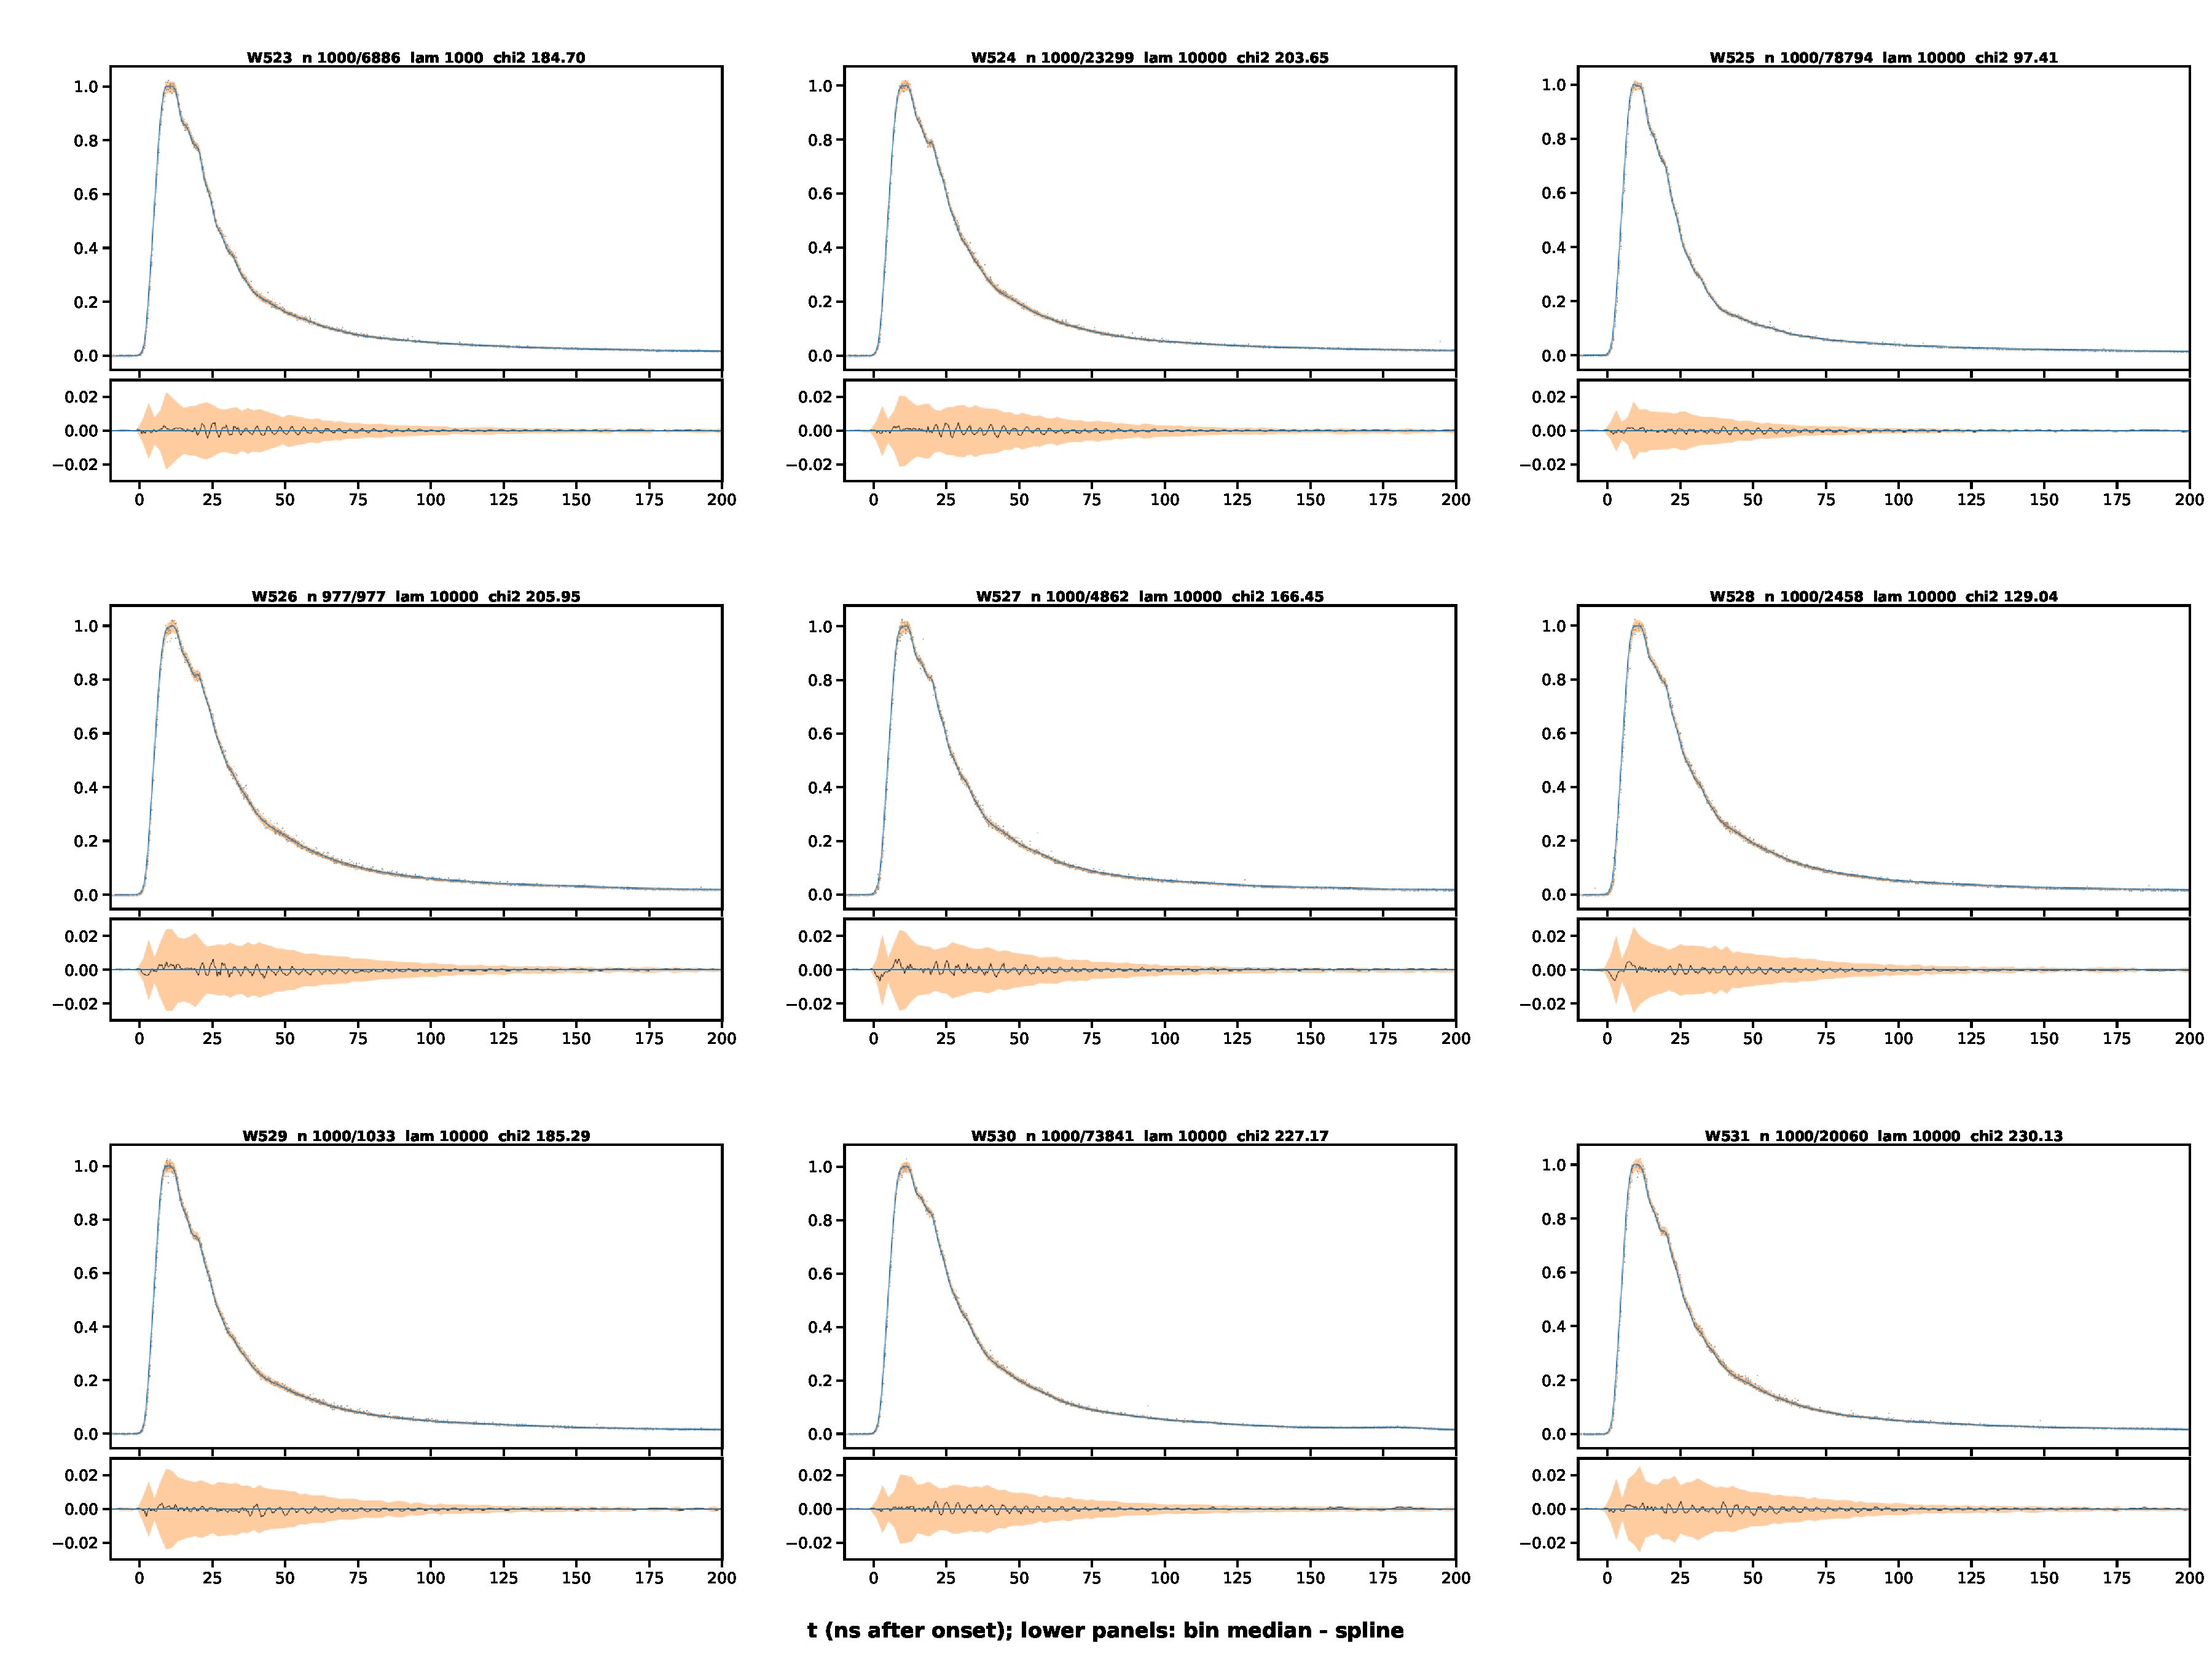
\includegraphics[width=\textwidth]{template_w526_elastic.pdf}
\caption{Templates of the innermost-ring modules W523 to W531 (\code{2p24GeV\_H2}, elastic pools). Upper panel per module: up to 3000 random pooled points $\tilde y_{ij}/v_{\max}$ on the final axis (grey dots), the spline $f$ (blue line) and the band $\pm$\code{shape\_sigma} (orange). Lower panel: bin median minus spline (black line) with the same band, on a $\pm 0.03$ scale. The abscissa is $t$ in ns after the onset, from $-10$ to 200\,ns. Each title gives $n_{\mathrm{pool}}/n_{\mathrm{pool,total}}$, $\lambda$ and the median $\chi^2/\mathrm{dof}$ of Eq.~\eqref{eq:chi2} over the kept pulses.}
\label{fig:grid_inner}
\end{figure}

\subsection{Outliers}

The only rejection is the \code{ok} test of Section~\ref{sec:align}. There is no $\chi^2$ cut and no sigma clipping; the spline fit is a plain weighted least squares on all points of the kept pulses, so a bad pulse that passes the test enters at full weight. Medians are used only in the bin statistics and the uncertainty estimators.

\subsection{Choice of the smoothing parameter}
\label{sec:lambda}

When the pool holds at least 10 pulses (\code{LAMBDA\_MIN\_POOL}) and a held-out set exists, the template is built for each $\lambda \in \{10^2, 10^3, 10^4\}$ (\code{LAM\_GRID}). The held-out pulses are aligned to each candidate template as in Section~\ref{sec:align}, and the chosen $\lambda$ minimises the mean, over the held-out pulses that are \code{ok} for every candidate that was built, of
\begin{equation}
\chi^2_{\mathrm{full},i}/\mathrm{dof} = \frac{1}{n_{\mathrm{win}} - 2} \sum_{j \in \mathrm{win}}
\frac{\big(y_{ij} - \hat A_i f(\tau_{ij})\big)^2}{\sigma_i^2 + \big(\hat A_i \sigma_t f'(\tau_{ij})\big)^2 + \big(\hat A_i \kappa f(\tau_{ij})\big)^2},
\label{eq:chi2full}
\end{equation}
the $\chi^2$ with the full point variance of Eq.~\eqref{eq:var} in amplitude units. If no held-out pulse is \code{ok} for all candidates, or the pool is smaller than 10 pulses, $\lambda = 10^3$ (\code{LAMBDA\_FALLBACK}).

For pools below 100 pulses (\code{OSC\_POOL\_MAX}) a wiggle check follows. On the 0.1\,ns output grid, the main peak is the largest value in $[3, 30]\ns$; any maximum or minimum of prominence at least $0.002$ of the peak value (\code{OSC\_PROM}) within $[2, 150]\ns$ (\code{OSC\_WIN}) and farther than 3\,ns from the main peak (\code{OSC\_EXCL}) counts as spurious. While any is found, $\lambda$ is multiplied by 10, capped at $10^4$ (\code{SMOOTH\_LAMBDA}), and the template rebuilt. A template still wiggly at $10^4$ counts as a failed fit, and the next pool of Section~\ref{sec:pools} is tried.

\section{Shape uncertainty}
\label{sec:unc}

\paragraph{Error of the mean shape.} \code{shape\_err} is $s_b / v_{\max}$ of the final pass, Eq.~\eqref{eq:sb}, interpolated onto the output grid and undefined (NaN) beyond $T_{\mathrm{data}}$. It is the statistical error of the template.

\paragraph{Pulse-to-pulse spread.} \code{shape\_sigma} is computed for every non-dead module, whether its template is its own or the fallback, and always from the amplitude band $200$ to $1000\adc$. Up to 1000 random band pulses are drawn with the generator seeded $(1, m, 1)$, a different draw from the general fit pool, and aligned to the module's final template as in Section~\ref{sec:align}. At least 50 aligned pulses must be \code{ok} (\code{SIGMA\_MIN\_POOL}). For every sample with $-8\ns \le \tau_{ij} \le T_{\mathrm{data}} - t_{\mathrm{on}}$ the residual and its noise variance are
\begin{equation}
R_{ij} = \frac{y_{ij}}{\hat A_i} - f(\tau_{ij}),
\qquad
\nu_{ij} = \frac{v_{\mathrm{ped}}\,(1 + 1/n_{\mathrm{ped}})}{\hat A_i^2},
\end{equation}
where $v_{\mathrm{ped}}$ is the mean over the pool of each pulse's sample variance at $\tau < -20\ns$ (\code{PRE\_ONSET\_NS}) and the factor $1 + 1/n_{\mathrm{ped}}$ adds the pedestal error. Here $f$ is the raw spline, which keeps its small pre-onset values, so the samples with $\tau \in [-8, 0]\ns$ are compared with them. In 2\,ns bins $b$ (\code{SIGMA\_BIN\_NS}) the spread $\sigma_b$ is the value $s \ge 0$ that solves
\begin{equation}
\median_{ij \in b} \frac{\big(R_{ij} - \median_b R\big)^2}{s^2 + \nu_{ij}} = 0.4549,
\label{eq:gsigma}
\end{equation}
the right-hand side being the median of a $\chi^2$ distribution with one degree of freedom (\code{CHI2\_1\_MED}). The equation is solved by 40 bisection steps; bins with fewer than 8 points (\code{SIGMA\_BIN\_MIN}) are NaN, and the bin values are linearly interpolated onto the output grid. With $\nu = 0$ the estimator reduces to $1.4826\,\MAD$; the noise is removed per point inside the median. \code{a\_band}, the median $\hat A_i$ of the band pool, records the amplitude at which the spread was measured.

\paragraph{Borrowed spread.} A module with fewer than 50 usable band pulses, or a dead module, gets \code{sigma\_borrowed} $= 1$ and receives, point by point, the median of \code{shape\_sigma} over all modules with their own value (the whole run type, all pool kinds), and the median of their \code{a\_band}. Figure~\ref{fig:grid_outer} shows outer modules, most of them with a borrowed spread.

\begin{figure}[htbp]
\centering
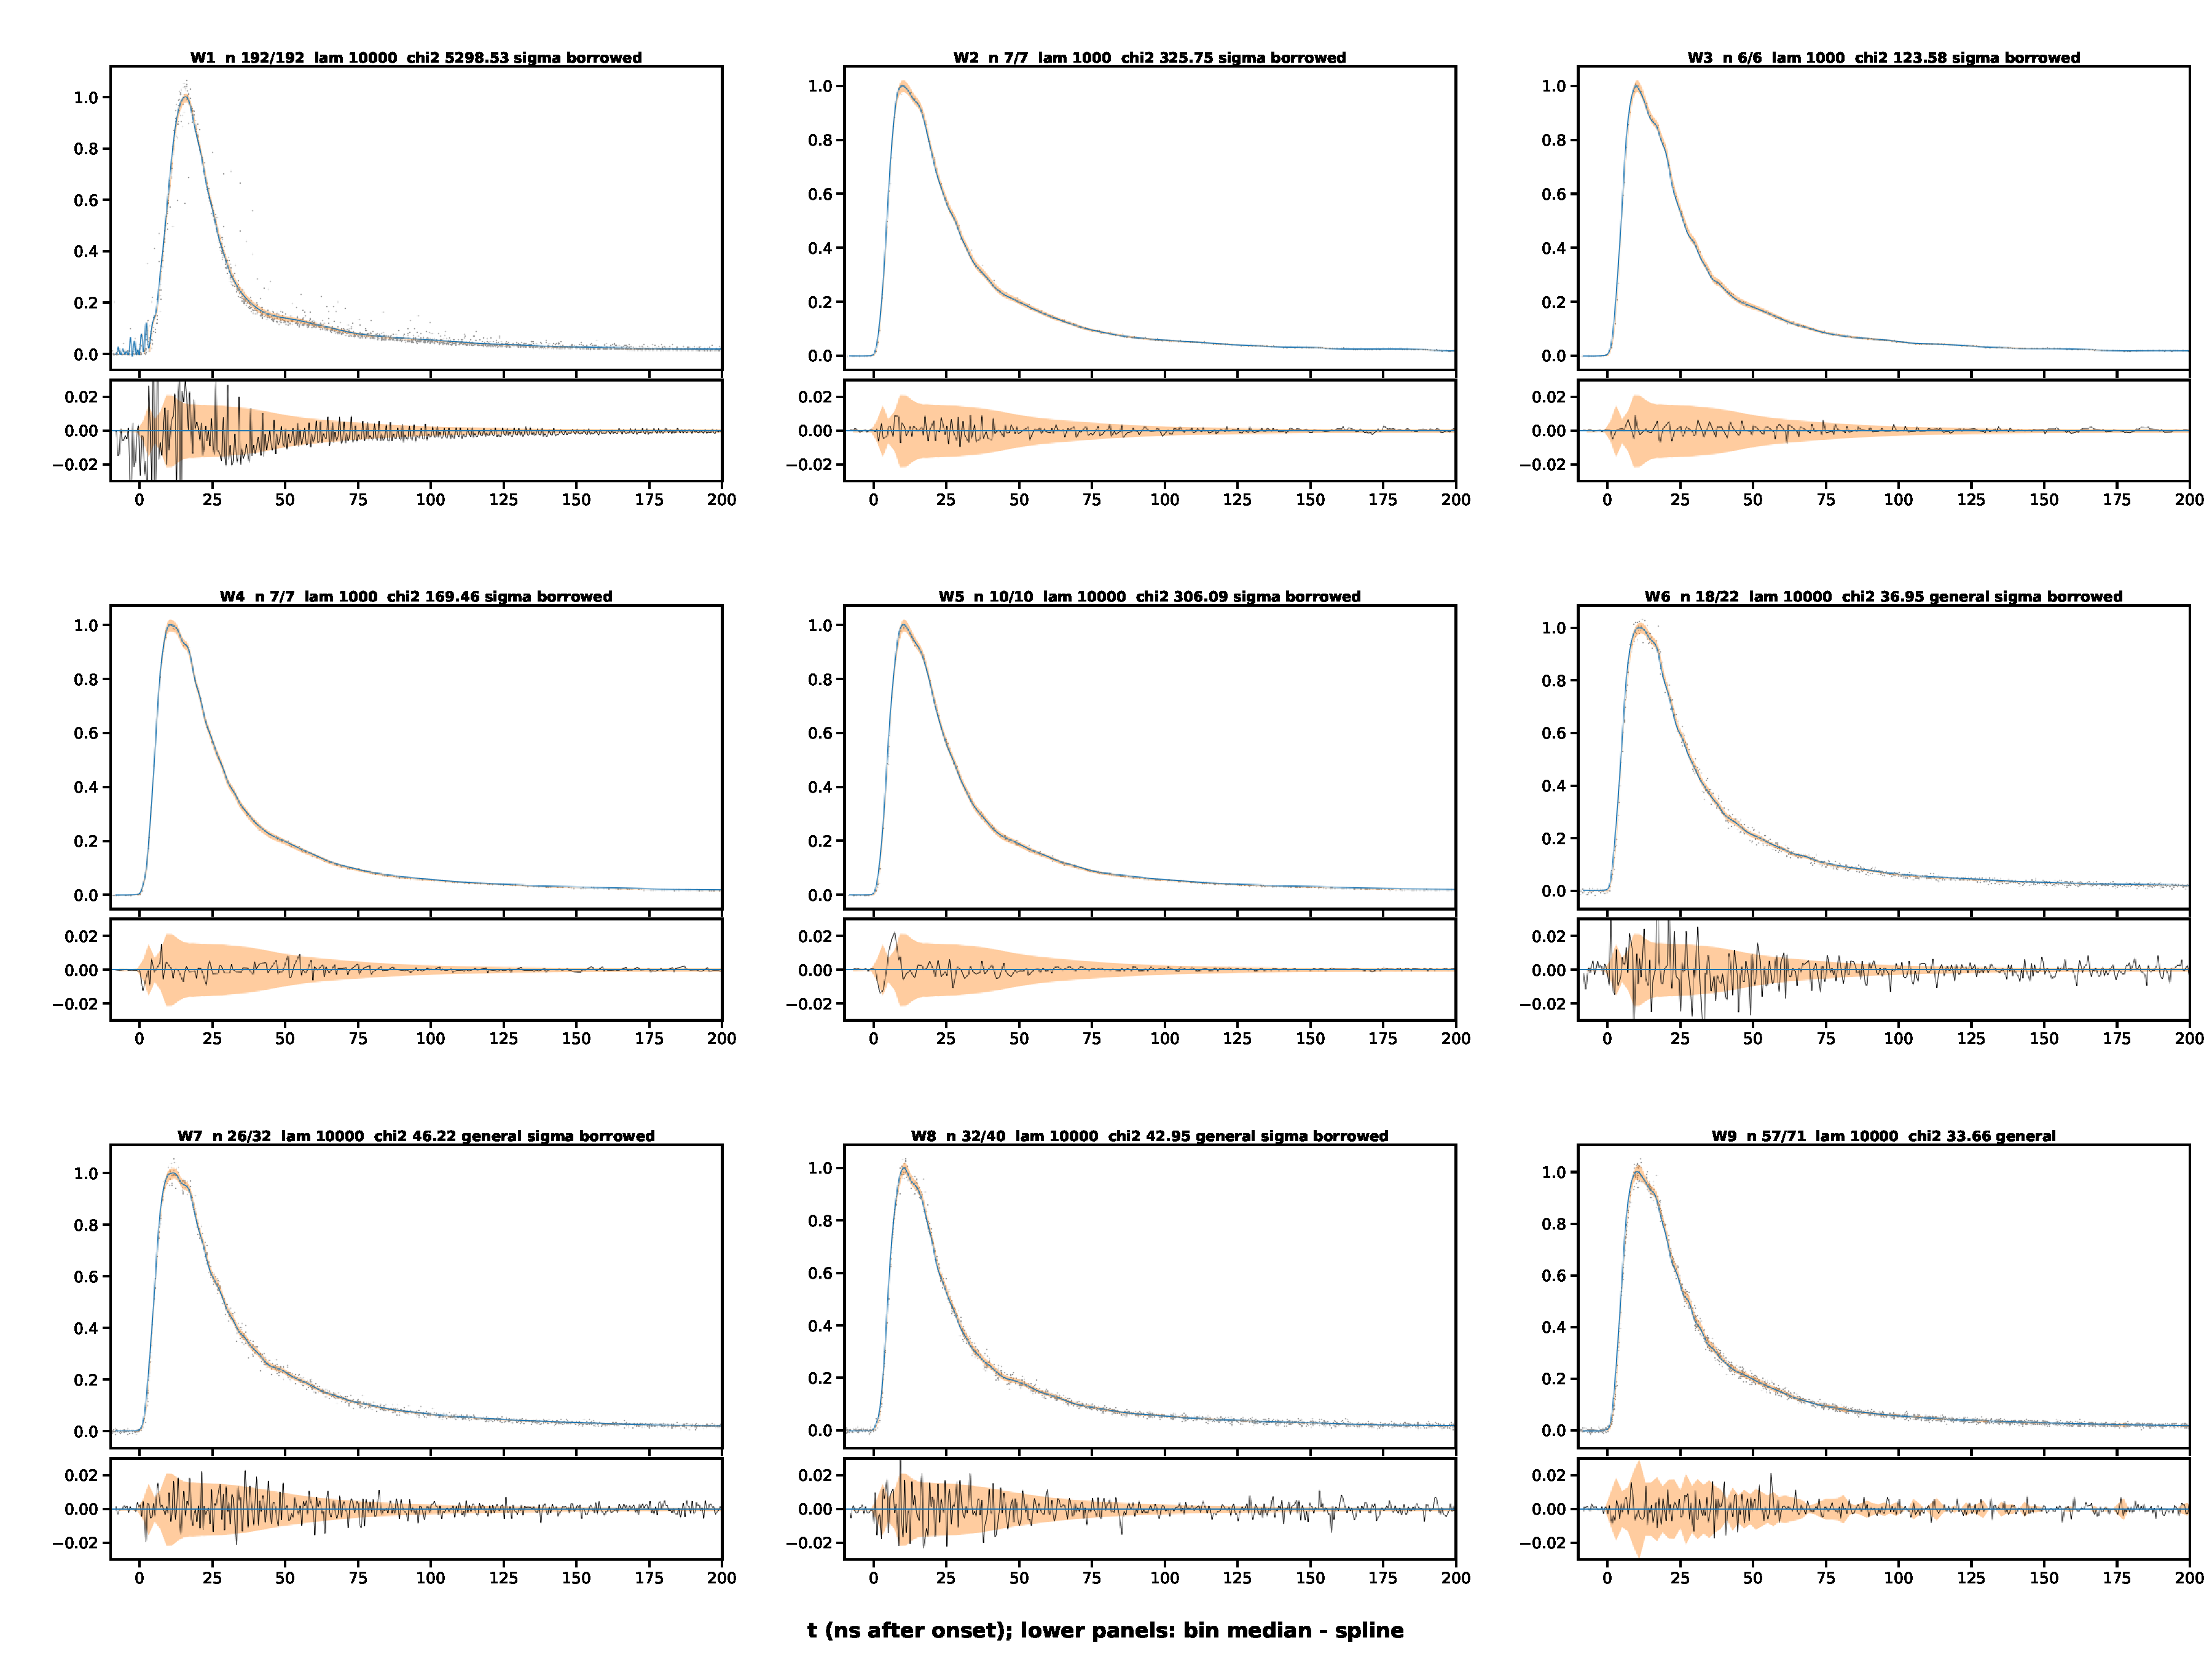
\includegraphics[width=\textwidth]{template_w6_general.pdf}
\caption{As Fig.~\ref{fig:grid_inner} for the outer modules W1 to W9 (\code{2p24GeV\_H2}). W1 to W8 have fewer than 50 usable band pulses and carry the borrowed spread (\code{sigma borrowed} in the title); W1 to W5 were fitted on elastic pools and W6 to W9 on general pools (\code{general}).}
\label{fig:grid_outer}
\end{figure}

\paragraph{Elastic spread.} \code{shape\_sigma\_elastic} applies the same estimator to the elastic fit pool about its own template, only when the template pool is elastic and holds at least 50 pulses; it is NaN otherwise.

\section{Fallback and run-type average}
\label{sec:fallback}

A module without its own template receives the run-type average; the \code{fallback} flag of the output takes the values 0 (own template) and 2 (run-type average), with no intermediate level implemented. The run-type average is built with the procedure of Section~\ref{sec:fit} at $\lambda = 10^4$ (\code{SMOOTH\_LAMBDA}) on up to 20 random kept pulses from every module with an own template from an elastic or single pool (the general-pool templates are excluded), drawn with the generator seeded $(1, 987654321)$. It runs the same alignment iteration, with no $\lambda$ scan and no wiggle check. Figure~\ref{fig:grid_avg} shows a module that received the average.

\begin{figure}[htbp]
\centering
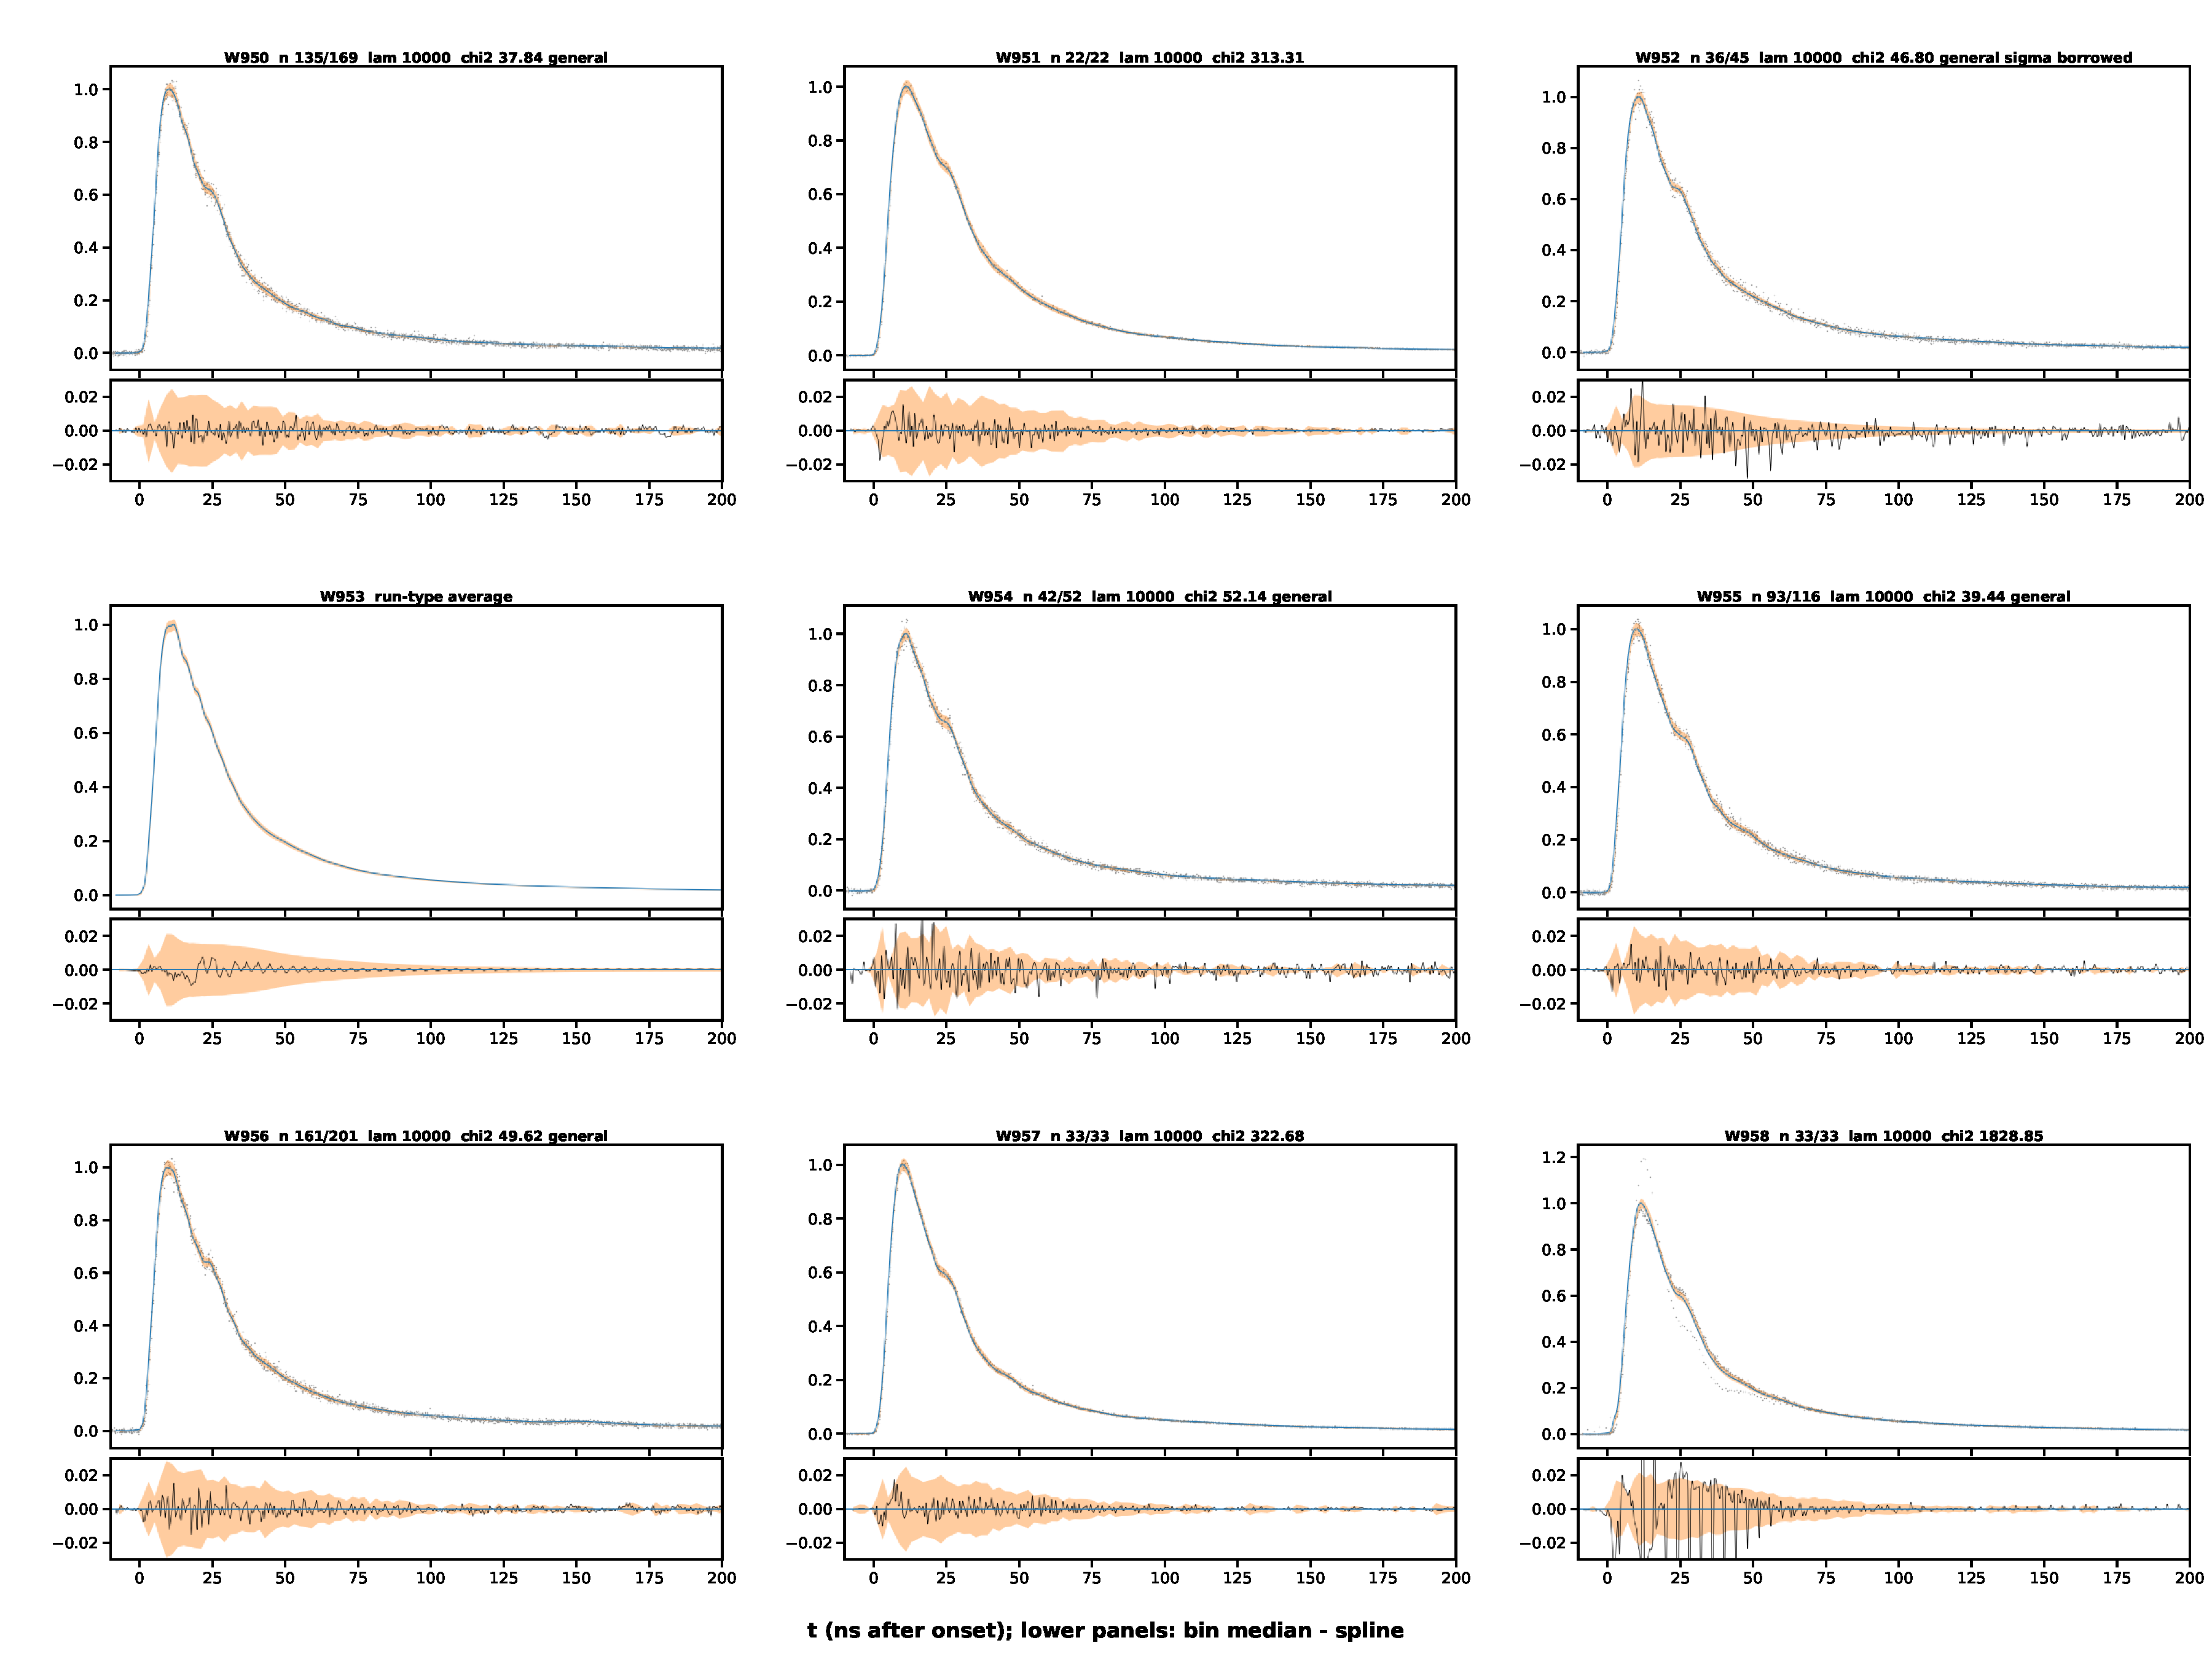
\includegraphics[width=\textwidth]{average_template.pdf}
\caption{As Fig.~\ref{fig:grid_inner} for the modules W950 to W958 (\code{2p24GeV\_H2}). W953 received the run-type average (\code{run-type average} in the title): its panels show the average shape, the borrowed \code{shape\_sigma} band and the residual of the average build, without pooled points. The other modules show their own fits.}
\label{fig:grid_avg}
\end{figure}

\section{Outputs and use of the template}
\label{sec:outputs}

The build writes \code{templates\_<RT>.npz} (schema \code{spline\_templates\_v3}), a ROOT file with a per-module tree of the main fields (knots, coefficients, shapes, flags, $\lambda$, \code{chi2\_ndf}, \code{a\_band}), and a PDF of diagnostic pages. Table~\ref{tab:outputs} lists the per-module content. The spline is stored on the final axis, with $t = 0$ at the 0.5\,\% onset and unit peak; the sampled shapes are given on the output grid \code{t\_grid} from $-8$ to 400\,ns in 0.1\,ns steps (\code{GRID\_DT}). In the ROOT file each module also carries a \code{TH1D} of the shape with \code{shape\_sigma} as bin errors.

\begin{table}[htbp]
\centering
\caption{Per-module content of the template file.}
\label{tab:outputs}
\small
\begin{tabular}{p{0.44\textwidth}p{0.50\textwidth}}
\toprule
Field & Content \\
\midrule
\code{spline\_k}, \code{spline\_t}, \code{spline\_c} & degree 3, knots and coefficients, NaN-padded to a common length \\
\code{spline\_nt}, \code{spline\_nc} & true lengths of the knot and coefficient arrays \\
\code{shape}, \code{shape\_err} & template and error of the mean shape on \code{t\_grid} \\
\code{shape\_sigma}, \code{shape\_sigma\_elastic} & pulse-to-pulse spread, band pool and elastic pool \\
\code{a\_band} & median fitted amplitude of the band pool (ADC) \\
\code{onset\_shift\_ns} & final axis minus CFD axis \\
\code{lam\_module} & smoothing parameter used \\
\code{chi2\_ndf} & median of Eq.~\eqref{eq:chi2} over the kept pulses \\
\code{align\_rms\_ns} & alignment rms of the last realignment \\
\code{n\_pool}, \code{n\_pool\_total} & pool size used; candidate count before the cap (elastic) or band size (general) \\
\code{dead}, \code{fallback}, \code{single}, \code{pool\_general}, \code{sigma\_borrowed} & flags \\
\code{t\_pk}, \code{t50} & peak time and half-maximum time of the template (ns) \\
\code{avg\_spline\_t}, \code{avg\_spline\_c} & run-type average spline (one per file) \\
\code{meta} & build record (constants, inputs, git revision) \\
\bottomrule
\end{tabular}
\end{table}

Each one-pulse overlay of the diagnostic pages draws $\hat A_i\, f(t - \hat t_{0,i})$ for $t > \hat t_{0,i}$ over the raw $y_{ij}$, using the final onset and amplitude of the pulse. A single-pulse fit with the template has two free parameters, $t_0$ and $A$, determined by the unweighted least squares of Eqs.~\eqref{eq:t0} and following over $\tau \in [-20, 160]\ns$, with the shape fixed. Figures~\ref{fig:ex_inner} and \ref{fig:ex_outer} show such overlays for an innermost-ring and an outer module.

\begin{figure}[htbp]
\centering
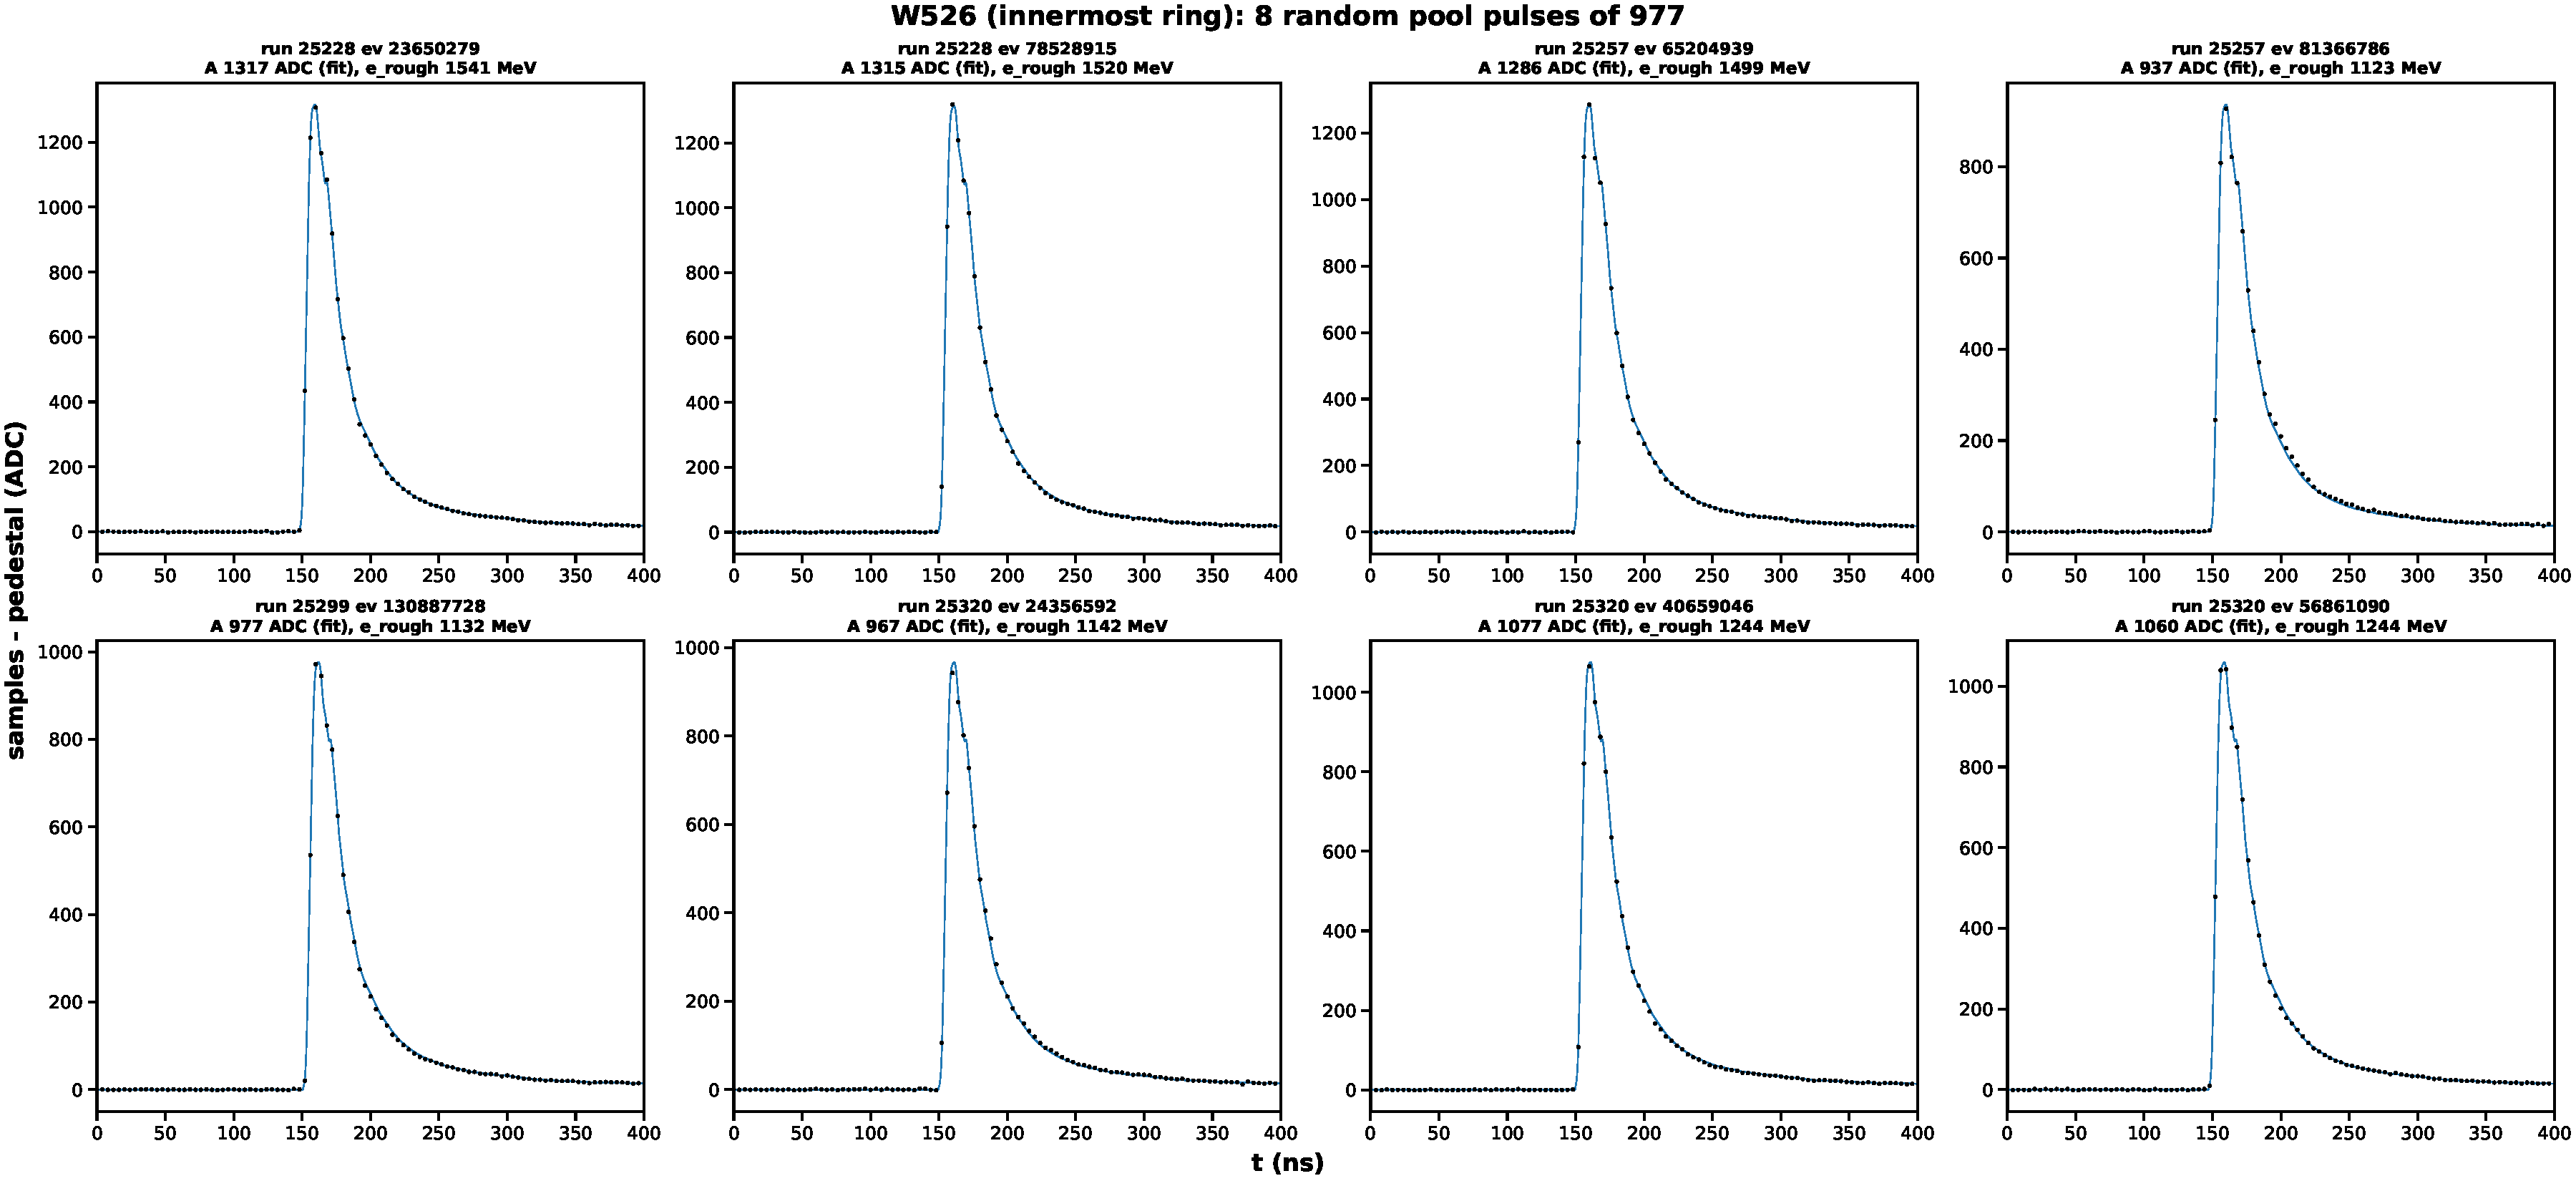
\includegraphics[width=\textwidth]{example_w526_innermost.pdf}
\caption{Eight random pool pulses of W526 (innermost ring, 977 pool pulses, \code{2p24GeV\_H2}). Black dots: pedestal-subtracted samples (ADC) at the 4\,ns sample times; blue line: $\hat A_i\, f(t - \hat t_{0,i})$ on a 0.5\,ns grid, zero for $t \le \hat t_{0,i}$, with the final onset and amplitude of the build. Each title gives the run and event number, the fitted amplitude and $e^{\mathrm{rough}}$.}
\label{fig:ex_inner}
\end{figure}

\begin{figure}[htbp]
\centering
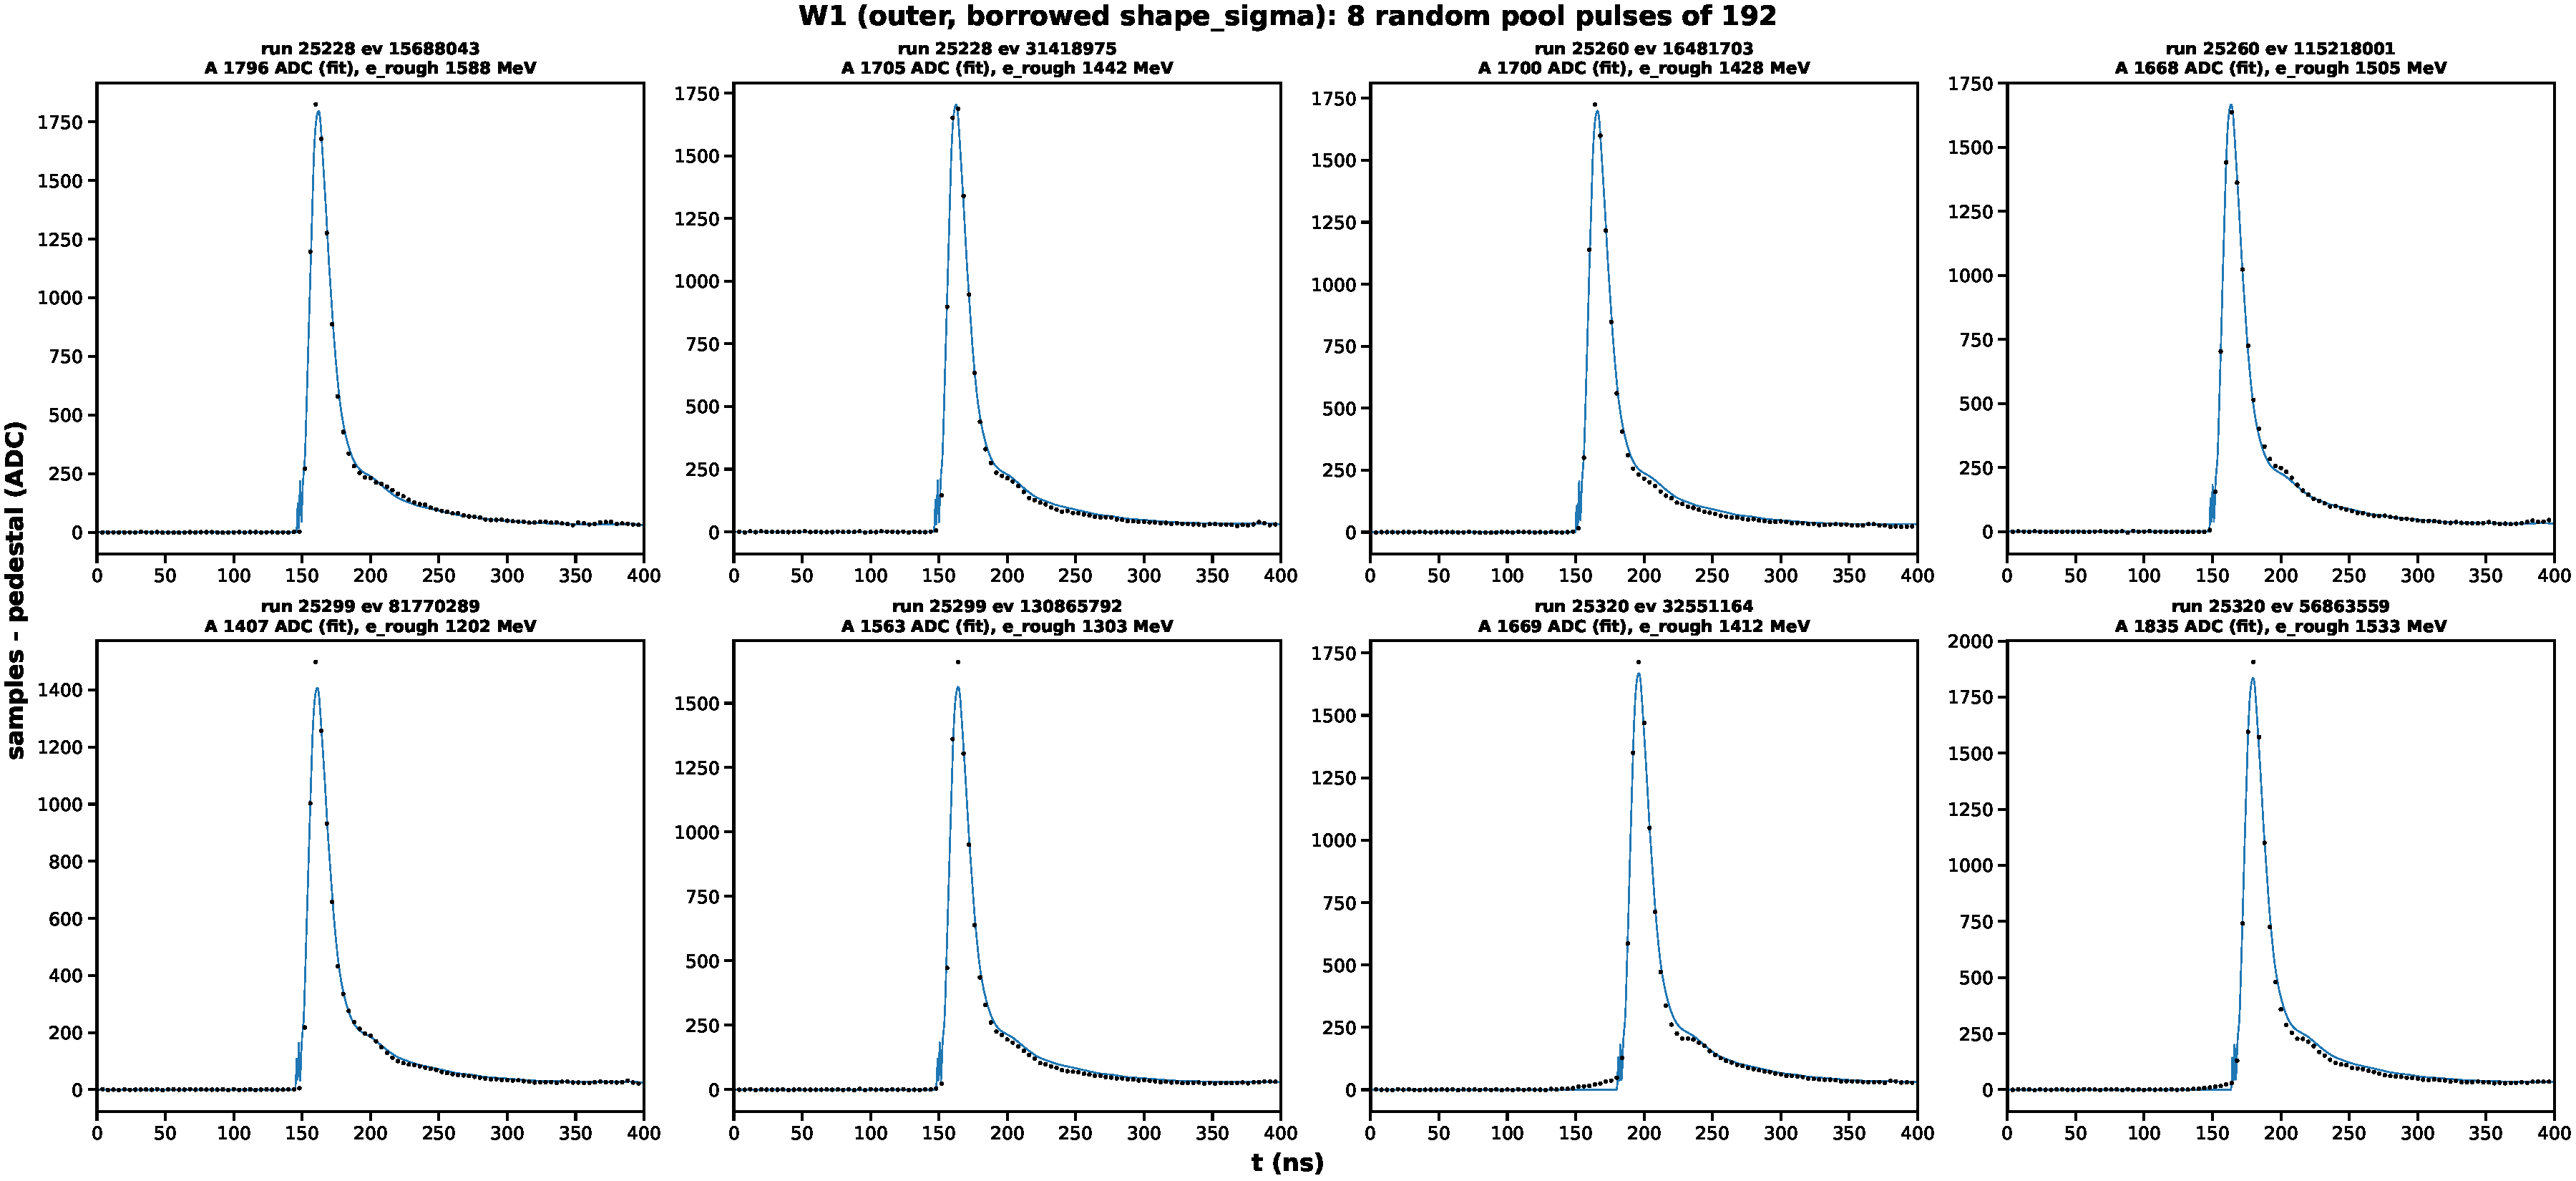
\includegraphics[width=\textwidth]{example_w1_borrowed.pdf}
\caption{As Fig.~\ref{fig:ex_inner} for W1 (outer module with a borrowed spread, 192 pool pulses).}
\label{fig:ex_outer}
\end{figure}

\section{Example build}

For the run type \code{2p24GeV\_H2} (numbers from the build log and the npz of that build): 1146 modules received their own template (136 from a general pool, 5 from a single pulse) and 6 the run-type average, 3 of them dead. The median pool size was 86 and 148 modules reached the 1000-pulse cap; 544 modules used the 87-knot plan and 602 the 76-knot plan. The chosen $\lambda$ was $10^2$ for 184 modules, $10^3$ for 148 and $10^4$ for 814. The median alignment rms per pass was 0.101, 0.108 and 0.115\,ns. The run-type average used 19\,502 pulses, and 98 own-template modules borrowed their \code{shape\_sigma}. Figure~\ref{fig:summary} is the summary page of that build.

\begin{figure}[htbp]
\centering
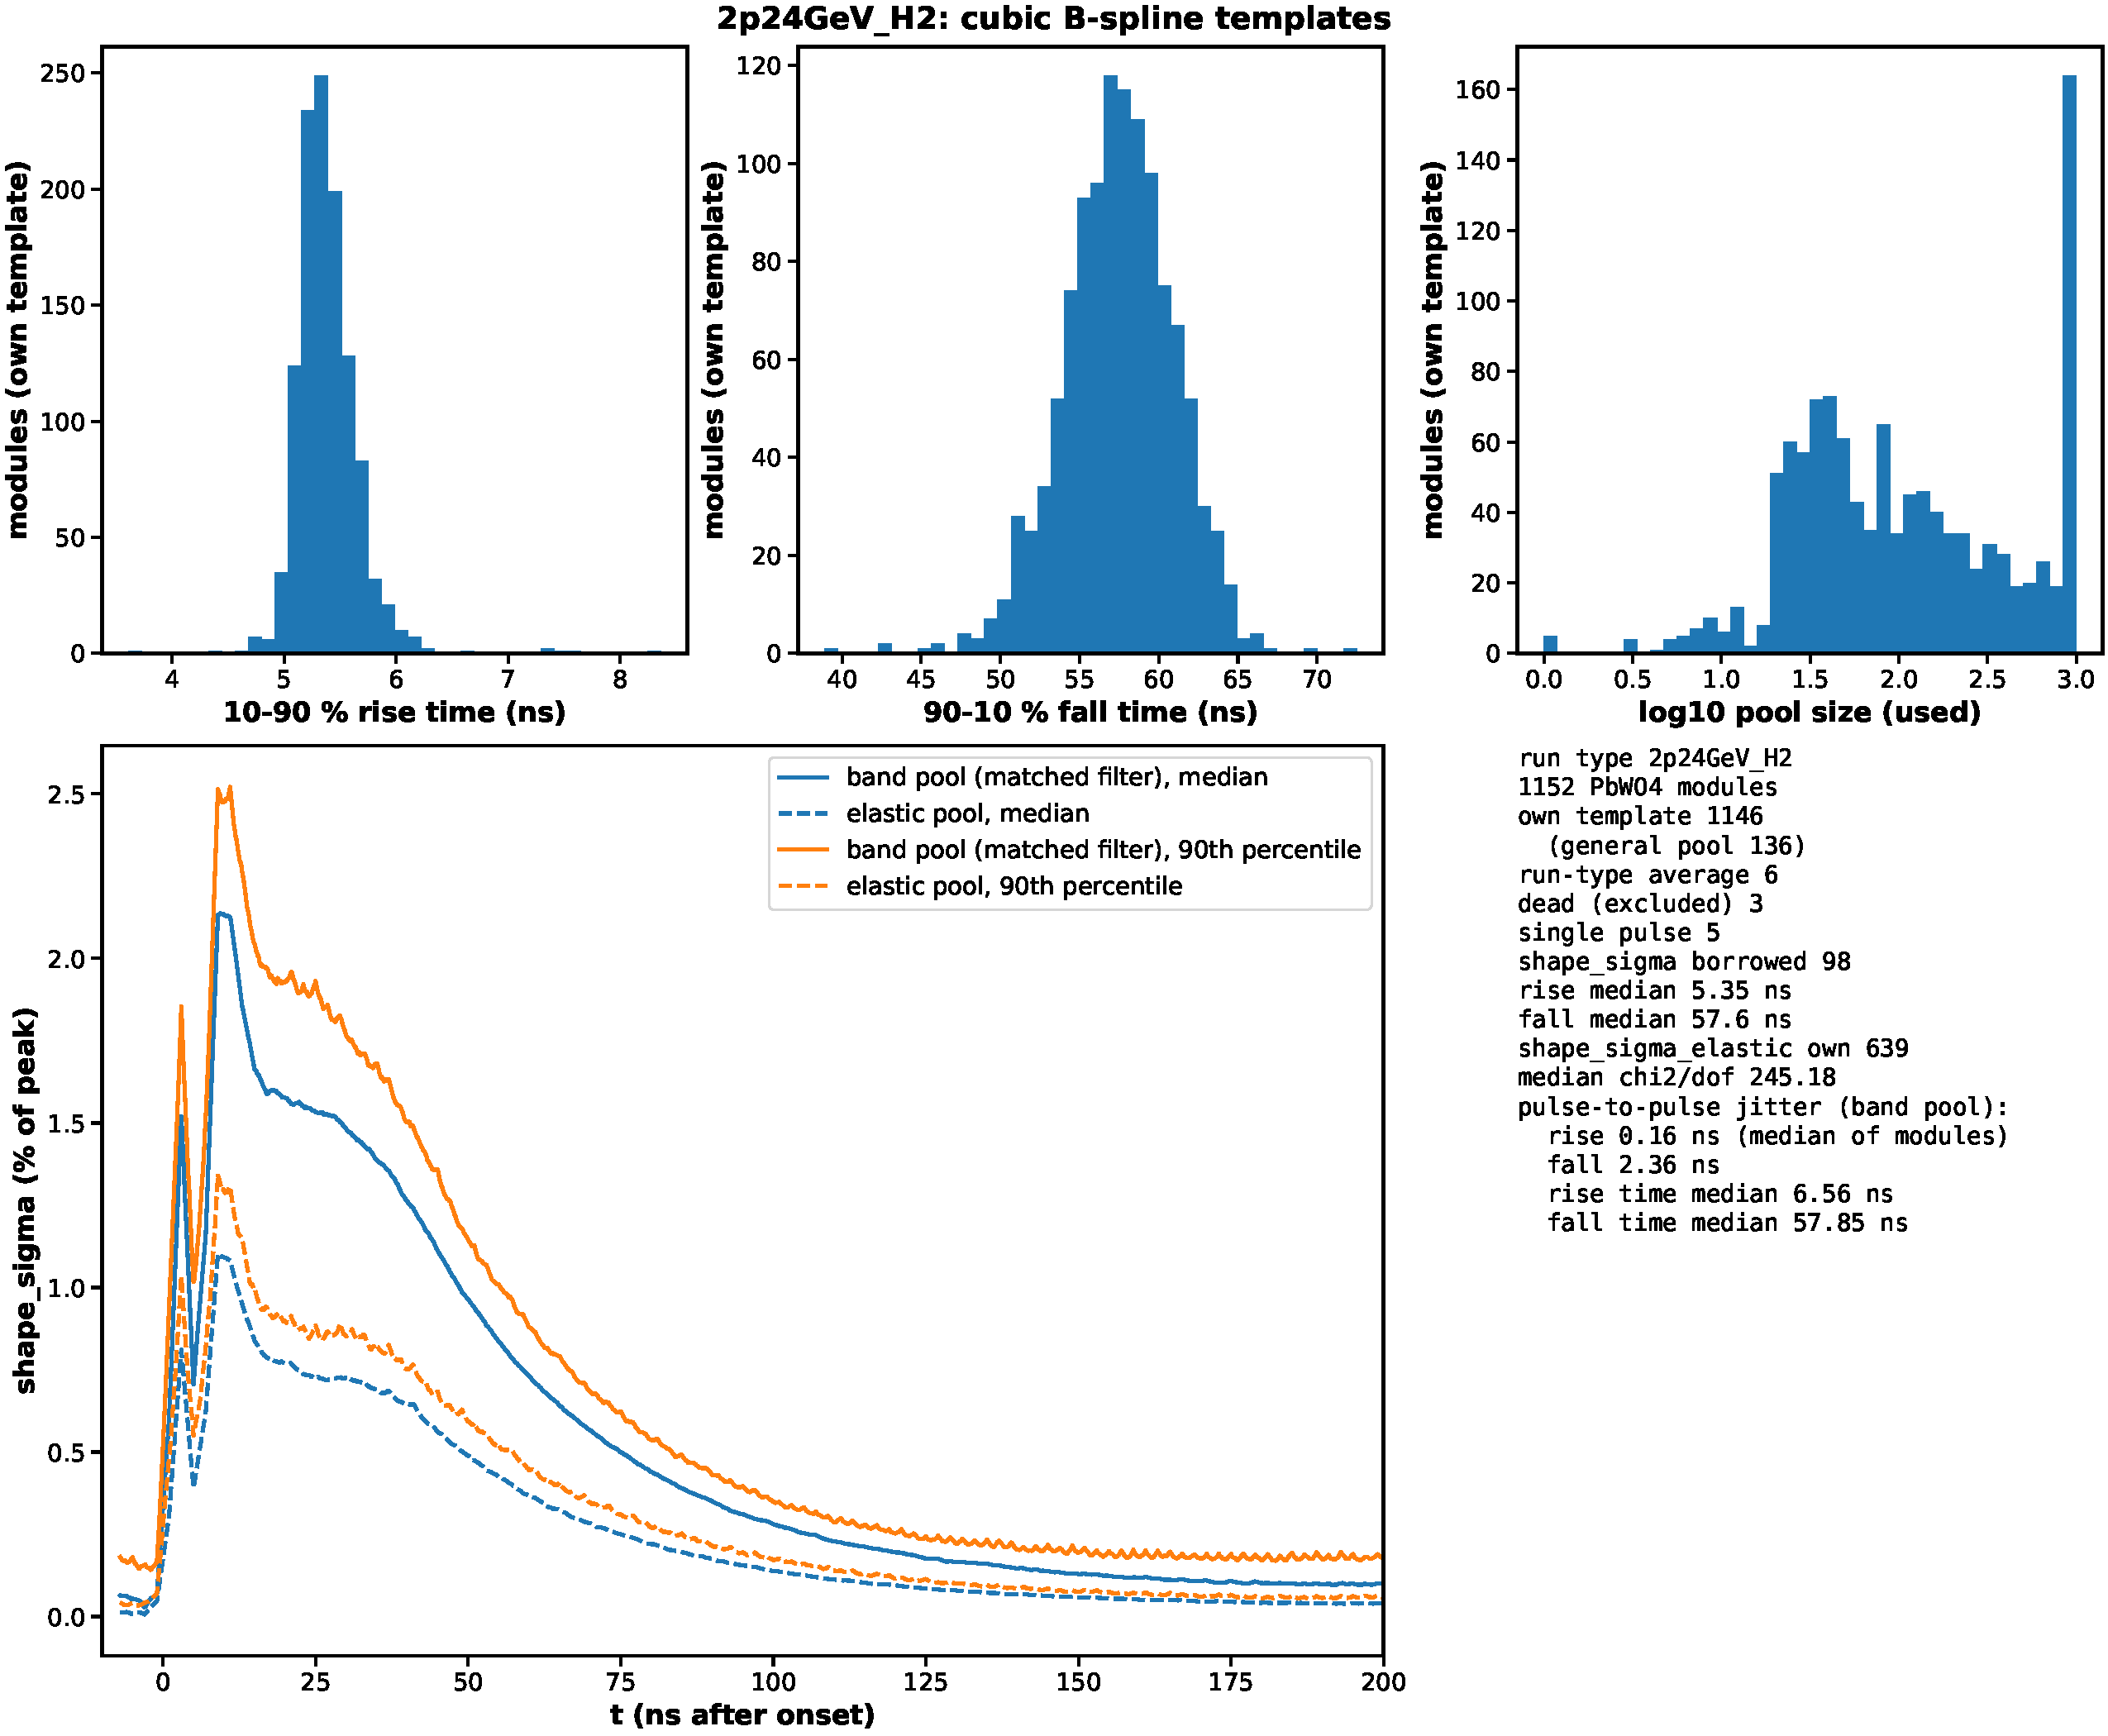
\includegraphics[width=\textwidth]{summary_overview.pdf}
\caption{Summary page of the \code{2p24GeV\_H2} build. Top row: histograms over the own-template modules of the 10--90\,\% rise time and the 90--10\,\% fall time of the template and of $\log_{10}$ of the pool size. Bottom left: \code{shape\_sigma} in percent of the peak versus $t$ for the modules with their own value, the band pool as solid lines and the elastic pool dashed; blue is the median over modules and orange the 90th percentile. Bottom right: module counts and medians of the build.}
\label{fig:summary}
\end{figure}

\end{document}
